\documentclass[12pt,a4paper]{article} % Defines the document as an article with 12pt font on A4 paper
\usepackage[utf8]{inputenc} % Sets UTF-8 encoding
\usepackage{geometry} % Enables page geometry customization
\geometry{margin=1in} % Sets 1-inch margins
\usepackage{graphicx} % Allows inclusion of images
\usepackage{titlesec} % Controls section formatting
\usepackage{hyperref} % Enables hyperlinks
\usepackage{tikz}
\usepackage{float}
\usepackage{pdflscape}
\usepackage{amsmath}
\usepackage{pgfgantt}
\usetikzlibrary{shapes.geometric, calc, arrows.meta, positioning}
\usepackage{setspace} % Allows line spacing adjustments
\usepackage{csquotes} % Improves quotation handling
\usepackage{datetime} % Provides date and time formatting
\usepackage{enumitem}
\usepackage[backend=biber,style=apa, sorting=nyt]{biblatex} % Configures bibliography using Biber with APA style
\addbibresource{references.bib} % Adds a bibliography file (replace with your .bib file name)
\renewcommand{\dateseparator}{-} % Sets date separator as '-'
\onehalfspacing % Sets line spacing to 1.5


\title{\textbf{Research Proposal: PhD candidate in Industrial Engineering}} % Defines the title
\author{
	\textbf{Benjamin R. Berton}\\
	Polytechnique Montréal\\
	\href{mailto:benjamin.berton@polymtl.ca}{benjamin.berton@polymtl.ca}\\
	\textit{Supervised by: Philippe Doyon-Poulin}
} % Defines author details

\begin{document} % Begins the document
	\maketitle % Generates the title
	
	\begin{center}
		\textbf{A cognitive modelling approach to evaluating Human-Autonomy Teaming in commercial aviation}
	\end{center} % Centers the research title
	
	\begin{center}
		Submitted to members of the Jury:\\
		Pr. Jean-Marc Frayret, Pr. Philippe Doyon-Poulin \& Pr. Shi Cao\\
		\date{\today} % Inserts today's date
	\end{center} % Centers the research title
	
	\newpage % Starts a new page
	
	\tableofcontents % Generates the table of contents
	\newpage % Starts a new page
	
	\section{Trigger \textbf{TBD}} % Defines a section titled "Trigger"
	Commercial aviation has shown a trend toward crew reduction, progressively decreasing the number of members in the cockpit \parencite{harris_human-centred_2007}. Historically, flight crews included up to five members, but technological advancements have reduced this number to two—the Captain (CPT) and First Officer (FO)—eliminating the need for flight engineers, navigators, and radio operators.
	
	Currently, the Federal Aviation Administration (FAA) - Part 25 regulations mandate a minimum of two pilots in the cockpit. However, technological advancements suggest the possibility of transitioning to Single Pilot Operations (SPO), where only one pilot would be on duty, assisted by advanced onboard technologies and potentially ground support \parencite{bilimoria_conceptual_2014}. While this transition is technically feasible, it introduces significant challenges, far more complex than previous crew reductions \parencite{matessa_using_2017}.
	
	One of the main issues with SPO is the removal of a redundancy layer, a fundamental element of aviation safety. Shifting from a two-pilot cockpit to a single-operator model requires ensuring an equivalent or higher level of safety compared to current operations \parencite{boy_requirements_2014}. Simply replacing the human co-pilot with increased automation is not a viable solution. Future operational concepts must rethink task distribution between the pilot and autonomy to maintain reliability and resilience.
	
	A key factor for the success of SPO is the collaborative aspect between humans and advanced automated systems, known as Human-Autonomy Teaming (HAT). This approach emphasizes effective cooperation between the single pilot and advanced autonomous systems, where these systems do more than assist—they act as teammates \parencite{shively_autonomy_2017}.
	
	HAT is based on the evolution from automation to autonomy. Automation refers to technologies that process data, make decisions, and execute tasks based on predefined procedures \parencite{hoff_trust_2015, hancock_imposing_2017}. Autonomy, on the other hand, refers to a system's ability to perform tasks with minimal human intervention over an extended period \parencite{endsley_here_2017, holbrook_enabling_2020}. This progressive shift toward greater autonomy fundamentally changes the human-automation relationship, evolving from simple interaction to genuine teamwork \parencite{endsley_here_2017}.
	
	However, increasing automation levels also presents challenges, particularly automation complacency, where excessive reliance on automated systems can lead to reduced vigilance and an inability to react effectively in case of anomalies \parencite{lee_design_2023}. To avoid this pitfall, it is crucial to design systems that promote active collaboration between the pilot and onboard autonomy \parencite{endsley_here_2017}. The goal of HAT is to ensure smooth and efficient cooperation, where autonomous systems act as real teammates, contributing to safer and more effective flight operations \parencite{mcneese_chapter_2020}.

	Recently, the European Union Aviation Safety Agency (EASA) published a concept paper that offers initial practical guidance for the application of artificial intelligence in aviation contexts \parencite{easa_guidance_2024}. The purpose of this document is to provide stakeholders with early insight into regulatory expectations concerning the integration of AI solutions in commercial aviation. This concept paper will serve as a key reference throughout the present proposal, particularly Section C.4, which addresses human factors in AI and aligns closely with Human-Autonomy Teaming (HAT) concepts relevant to this thesis, where applicable, EASA objectives will be referenced to show how this research is trying to comply with regulations' guidance for AI-systems development.

	\section{Theoretical Background}
	\subsection{Human-Autonomy Teaming}

	Human-Autonomy Teaming (HAT) refers to the design and implementation of autonomous systems that work alongside human operators as collaborative teammates, rather than as mere tools or passive assistants. The concept emerges from the broader trajectory of automation in complex systems such as aviation, which has progressively shifted from manual control partially automated and now increasingly autonomous operations.

	Traditionally, automation has been defined as the execution of predefined rules to support or replace specific functions previously handled by humans \parencite{parasuraman_model_2000,hancock_imposing_2017,hoff_trust_2015}. Autonomy, in contrast, implies the capability of systems to make independent decisions,and adapt to context over extended periods with minimal human intervention \parencite{endsley_here_2017-1,holbrook_enabling_2020}. This evolution from automation to autonomy marks a fundamental transformation in human-system relationships: from simple interactions to teamwork \parencite{endsley_here_2017-1}.

	HAT is not only about increasing system autonomy, but also about enabling forms of \textbf{interdependence, coordination, and communication} that reflect the qualities of high-performing human teams. In the context of Single Pilot Operations, where traditional crew redundancy is removed, HAT systems must be designed to fill this critical gap — supporting the pilot while maintaining overall system resilience and safety \parencite{mcneese_chapter_2020}.

	Several key tenets have been identified as necessary for successful HAT \parencite{wynne_integrative_2018}:

	\begin{itemize}
		\item \textbf{Agency:} The autonomy must possess the authority and ability to act independently, initiate actions, and respond dynamically to changing contexts. Without agency, the system cannot be considered a true teammate.
		
		\item \textbf{Bidirectional Communication:} Effective teaming requires shared language and mutual intelligibility. The human and the autonomy must be able to exchange information, negotiate roles, and clarify intent. This includes both transparency of the autonomous system and user-directed interfaces \parencite{christoffersen_1_2002,liu_cognitive_2016}.
		
		\item \textbf{Shared Mental Models:} Team members must maintain compatible internal models of the task environment and of each other's roles and expectations. Shared mental models facilitate coordination and mutual predictability \parencite{cooke_interactive_2013,liu_cognitive_2016}.
		
		\item \textbf{Shared Intent:} Beyond tasks and states, effective teaming requires the communication of goals and future plans. This supports alignment and enables each teammate to anticipate and adapt to the other's behavior \parencite{lyons_humanautonomy_2021,endsley_ironies_2023}.
		
		\item \textbf{Interdependence:} Effective teams rely on one another. In HAT, this means distributing responsibilities based on respective strengths, with the autonomy taking on tasks that reduce workload or increase redundancy, while still enabling human oversight and intervention \parencite{lawless_editorial_2023,johnson_no_2019}.
	\end{itemize}

	Ultimately, the aim of HAT is to enable safer and more resilient socio-technical systems through intelligent teamwork. In the following sections, we explore the concept of Situation Awareness (SA) and its relevance to evaluating teaming interactions.

	\subsection{Situation Awareness}

	Situation Awareness (SA) is a foundational construct in human factors engineering in dynamic, safety-critical domains such as aviation. SA has become one of the most widely adopted models for understanding and assessing individuals and teams in complex operational settings. SA refers to the individual's capacity to perceive, interpret, and anticipate elements in the environment relevant to task goals.

	Endsley's three-level model of SA \parencite{endsley_measurement_1995} remains the most widely used framework and defines SA as follows:
	\begin{enumerate}
		\item \textbf{Level 1 - Perception:} The detection and identification of critical elements in the task environment. This includes sensory input, sensor data, displays, and communications that provide the operator with a raw understanding of “what is happening.”
		
		\item \textbf{Level 2 - Comprehension:} The integration and interpretation of perceived elements into a coherent mental model. At this level, the operator understands the significance of the information in relation to task goals and constraints.
		
		\item \textbf{Level 3 - Projection:} The ability to anticipate future states of the environment based on current comprehension. This level supports proactive decision-making, enabling the operator to stay ahead of unfolding events.
	\end{enumerate}

	These three levels represent a cumulative process. Operators typically must perceive relevant data (Level 1) before they can comprehend their meaning (Level 2) and ultimately project future developments (Level 3). The quality of SA is therefore sensitive to information availability, interface design, and attentional limitations \parencite{endsley-2015}.

	SA is highly predictive of human performance in complex environments and has been repeatedly identified as a root factor in accidents and near misses across domains \parencite{endsley_systematic_2021}. Its central role in safety and performance has led to extensive research in both assessment methods and system design principles that promote better SA in humans and, increasingly, in artificial agents \parencite{kokar_situation_2012}.

	In this context, SA is increasingly regarded not only as a human attribute but as a capability that autonomous systems must also demonstrate. Smart agents must be able to perceive relevant environmental cues, interpret task-relevant meaning, and anticipate future states to act appropriately and support the human operator. This shift is especially critical in Human-Autonomy Teaming (HAT), where autonomous systems are expected to share mental models, understand shared intent, and maintain alignment with human teammates.

	The following subsections will explore how SA extends to teams (Team SA) and how it can be formally represented and assessed within computational models.

	\subsubsection{Team-Situation Awareness}

	As we shift from analyzing individual performance to evaluating collaborative human-machine systems, the concept of Situation Awareness (SA) must also be extended to the team level. This is particularly critical in Human-Autonomy Teaming (HAT), where effective coordination depends on the distribution and alignment of SA across human and artificial agents.

	\textbf{Team SA} is defined as “the degree to which every team member has the SA required for his or her responsibilities” \parencite{endsley_measurement_1995}. In this view, each teammate—whether human or artificial—must possess an accurate and functional representation of the environment that supports the tasks they are responsible for. Numerous studies have shown that Team SA is a strong predictor of team performance across a variety of domains \parencite{cooke_measuring_2001,prince_measurement_2007,parush_individuals_2017}.

	A subset of Team SA, known as \textbf{Shared SA}, refers to “the degree to which team members possess the same SA on shared SA requirements” \parencite{endsley_designing_2003}. Because team roles often involve only partially overlapping responsibilities, shared SA pertains specifically to the common understanding of critical task-relevant information that must be aligned between teammates in order to enable effective coordination.

	In the context of HAT, these concepts are essential: both the human and the AI must possess correct SA for their respective tasks (Team SA), and they must also maintain alignment on overlapping task elements (Shared SA). For the autonomous agent, SA refers to an internal representation of the task environment that supports reliable, context-sensitive behavior. Moreover, the human operator must also maintain SA regarding the autonomous system—its state, capabilities, intentions, and limitations—and vice versa, especially when dynamic delegation, trust, and supervision are involved \parencite{endsley_designing_2003,national_academies_of_sciences_engineering_and_medicine_human-ai_2022}.

	To operationalize Team SA in HAT systems, \textcite{endsley_supporting_2023} recommend using Goal-Directed Task Analysis (GDTA) method which has been adapted to teams. This enables the identification of information requirements at all three levels of SA (perception, comprehension, and projection) for each role in the system, as well as the information that must be shared.

	In this research, Team SA serves as both a conceptual foundation and an evaluative criterion for comparing different teaming configurations. It offers a way to assess whether the human and AI are functionally aligned in their understanding of the situation and each other, which is a prerequisite for safe and effective operation in Single Pilot Operations (SPO) settings.

	The next section will examine how these concepts can be modeled computationally, through cognitive architectures that simulate the mechanisms underpinning SA in both human and artificial agents.

	\subsubsection{Computational models of Situation Awareness}

	Computational models of Situation Awareness (SA) offer a rigorous, theory-based approach for simulating and assessing the cognitive processes that underlie perception, comprehension, and projection in complex, dynamic tasks. These models aim to formalize SA as a measurable construct that can inform system design, interface optimization, and performance evaluation in both human and autonomous agents.

	Several approaches have emerged to model and predict SA quantitatively, especially within safety-critical domains such as aviation. One prominent family of models builds upon the \textbf{SEEV framework} (Salience, Effort, Expectancy, and Value), which predicts visual attention distribution based on environmental and task-related factors. \textcite{wang_real-time_2024} proposed a real-time measurement model of attention allocation grounded in SEEV, validated in a low-fidelity Single Pilot Operation (SPO) flight deck scenario. Their study demonstrated how fixation data and task performance differed between SPO and two-pilot configurations under engine failure conditions, highlighting the importance of interface design in shaping attention allocation and supporting level 1 SA.

	Building on attention modeling, \textcite{chen_developing_2021} integrated the ACT-R theory to develop an SA model to predict operator performance under different interface conditions. Their enhanced model used multiple data sources including SAGAT probes, eye-tracking data, and subjective ratings (10-D SART) to validate the predictive accuracy of the SA estimates at each of the three levels. The model's outputs showed strong correlations with actual performance metrics, reinforcing the potential of cognitively grounded SA models for cockpit evaluation and design optimization.

	\textcite{juarez-espinosa_situation_nodate} developed an ACT-R model capable of responding directly to SAGAT probes, reinforcing the utility of cognitive architectures for SA measurement—not just behavior emulation. This direct probing technique has been adopted in recent implementations such as QN-ACTR-SA, where model introspection mimics SAGAT-style assessments without disrupting task flow.

	The \textbf{QN-ACTR-SEEV framework}, as developed by \textcite{rehman_phd_thesis} provides a hybrid cognitive architecture that simulates both attention allocation and memory-based SA dynamics. This approach has been applied to driving environments, demonstrating its utility in modeling Level 1 SA. The SEEV component governs gaze behavior across predefined Areas of Interest (AOIs), while the ACT-R layer simulates information encoding, retrieval, and decay. Together, these components allow the model to estimate an agent's SA during simulated scenario, using information probes.

	Beyond attention and memory modeling, \textcite{freiman_assessing_2019} introduced a high-fidelity SA component within an autonomous synthetic teammate in a remotely piloted aerial system task. Developed in ACT-R, the AST included dedicated SA buffers to monitor and interpret teammate communication, task states, and environmental cues. The model's performance in joint missions was comparable to human-human teams, suggesting that cognitive fidelity in SA modeling can be used within an autonomous agent to align the team and achieve high performance.

	In parallel, fuzzy logic and probabilistic reasoning have also been used in SA modeling to handle uncertainty in agent perception and decision-making. A recent systematic review by \textcite{daniello_fuzzy_2023} highlights the growing adoption of fuzzy logic in SA systems, particularly in domains where cognitive architectures may fall short in representing ambiguity or imprecise goals.

	These computational approaches differ in fidelity, focus, and domain of application, but all converge on a shared goal: simulating the cognitive processed of SA to support system design, training, and evaluation. In this thesis, we adopt the QN-ACTR-SEEV model, validated in driving contexts as the foundation for a cognitively plausible simulation of pilot SA in Single Pilot Operation scenarios. This model allows us to estimate not only human SA, but also the alignment of situation representation in Human-Autonomy Teams, thus enabling rigorous assessment of \textbf{Team SA} and \textbf{Shared SA} across different teaming configurations.

	\subsection{Knowledge gap} % Section title "Knowledge Boundaries"
	
	%\section{Research Question and Hypothesis} % Section for research question and hypothesis
	%\textbf{Question:} How does introducing a virtual co-pilot based on a cognitive model influence pilot performance and situation %awareness in Single Pilot Operations?
	%
	%\textbf{Hypothesis:} A virtual co-pilot, designed with a rigorous cognitive model, improves pilot situation awareness while %reducing cognitive load.
	
	\section{Objectives} % Defines the "Objectives" section
	The general objective of this research is to develop a methodology that facilitates the design of an autonomous agent collaborating with a human pilot for commercial aviation operations. To do so, we will use a collection of methods from the human factors and ergonomics research domain, especially cognitive modelling of human level 1 Situation Awareness.

	The Autonomous Agent or AI Agent (AA) that we aim to develop will be able to perform automatic selection and implementation of actions, the single pilot will still maintain full oversight and override capability of the AA. This level of autonomy corresponds to the level 2 of the EASA taxonomy where there is a partial release of authority to the autonomous system, while the pilot remains consistently accountable for the operations.

	\paragraph{EASA Objective CL-01 -- Classify the AA, with adequate justifications} the HAT system will fall under Level 2A and 2B of EASA's Human-AI teaming framework see Figure~\ref{fig:easa-taxo}, wherein humans and AI agents work jointly toward a predefined, shared objective through a directive and co-constructive approach, respectively, to problem-solving. Collaboration, more than cooperation, requires the ability to share situation awareness and dynamically adapt strategies and task allocations in real time through effective communication. 

	Our research question is: \textit{"Can we use cognitive models to evaluate HAT design systematically?"}

	\begin{figure}[H]
		\centering
		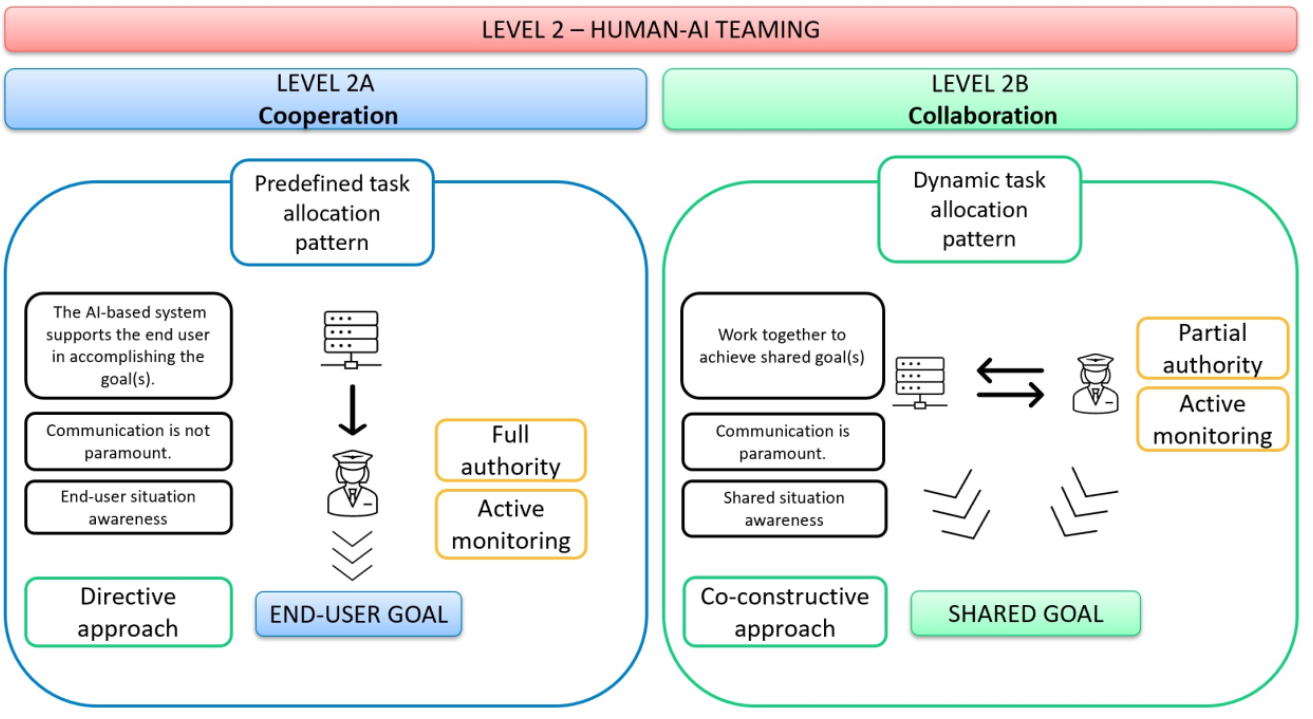
\includegraphics[width=1.0\textwidth]{./images/easa_taxo.png}
		\caption{HAT systems taxonomy as detailed in the EASA concept paper \parencite{easa_guidance_2024}}
		\label{fig:easa-taxo}
	\end{figure}
	
	To achieve this objective, the thesis will be comprised of three phases.
	\begin{enumerate}[label=\textbf{\arabic*.}]
		\item We will conduct a thorough analysis of the work and design domain in order to delineate the taskwork and teamwork and list requirements for the agent design. Especially:
		\begin{enumerate}[label=\textbf{\arabic{enumi}.\Alph*.}]
			\item \label{obj:1a} Identify the goal hierarchy that pilots use to achieve high levels of safety and performance in current day operations.
			\item \label{obj:1b} List the information required to construct a good Situation Awareness in the scenario 
		\end{enumerate}
		\item We will develop in parallel a cognitive model of the human pilot and a prototype of the AA, enabling them to interact in a closed-loop simulation environment. 
		\begin{enumerate}[label=\textbf{\arabic{enumi}.\Alph*.}]
			\item \label{obj:2a} Combine QN, ACT-R, and SEEV theory to create a cognitively plausible model of human pilot's perception of elements in the current situation (level 1 Situation Awareness)
			\item \label{obj:2b} Model the task using outputs from the GDTA and IA so that the cognitive model is capable of navigating the scenario on its own.
			\item \label{obj:2c} Develop an agent that can perform the tasks described in the IA.
			\item \label{obj:2d} Develop an Human-Agent Interface that comply with the teaming requirements established in the IA extend the cognitive model so that it can team-up with the autonomy to navigate the scenario.
		\end{enumerate}  
		\item We will conduct Human-In-The-Loop Simulation studies with expert pilots in order to :
		\begin{enumerate}[label=\textbf{\arabic{enumi}.\Alph*.}]
			\item \label{obj:3a} Validate the cognitive model
			\item \label{obj:3b} Investigates the human factors that weren't modeled such as trust in the autonomous agent and usability of the interface.
		\end{enumerate}
	\end{enumerate}
	These phases will be detailed in the next section 
	
	\section{Methodology} 

	\subsection{The operational scenario}
	The preliminary step for applying the methodology is to select a proper scenario, that is (1) realistic, so that information is easily available for modelling and knowledge gained can benefit the aviation industry, (2) challenging enough so that teaming with an autonomous agent is strongly beneficial for achieving good performance, and (3) procedural, deterministic, and short enough so that the cognitive modelling and agent implementation can realistically be implemented inside Polytechnique's flight simulator platform.
	
	The scenario consists in a takeoff and initial climb phase with an engine failure due to a bird or drone strike. The scenario is performed by a single pilot in a multi-engine very light jet aircraft, the Cessna Citation Mustang. Take-off with an engine failure is a challenging scenario for single pilot operations that is highly dynamic and requires fast and precise action taking from the captain. Bird and drone strike will be an issue for the foreseeable future of commercial aviation and is therefore a scenario of particular interest for the aviation industry.

	\paragraph{Objective CO-01 - Identify the list of end users that are intented to interact with the AA, together with their roles, responsibilities, indication of the level of teaming with the AA, and expected expertise.}
	\begin{itemize}
		\item The single pilot, with captain status is the primary end user that is intended to interact with the AA, its training on type, role and responsibilities remain unchanged compared to current-day single pilot operations. The captain is assumed to have been trained on using the AA, the captain will cooperate and collaborate with the AA.
		\item Air traffic controllers are secondary users of the AA. Their roles and responsibilities remain unchanged, they will not team with the AA. They are not assumed to have been trained on using the AA, they might simply receive a vocal message on the radio made by the AA and must act as if it was emitted by the human pilot. 
	\end{itemize}
	
	\begin{figure}[H]
 		\centering
  		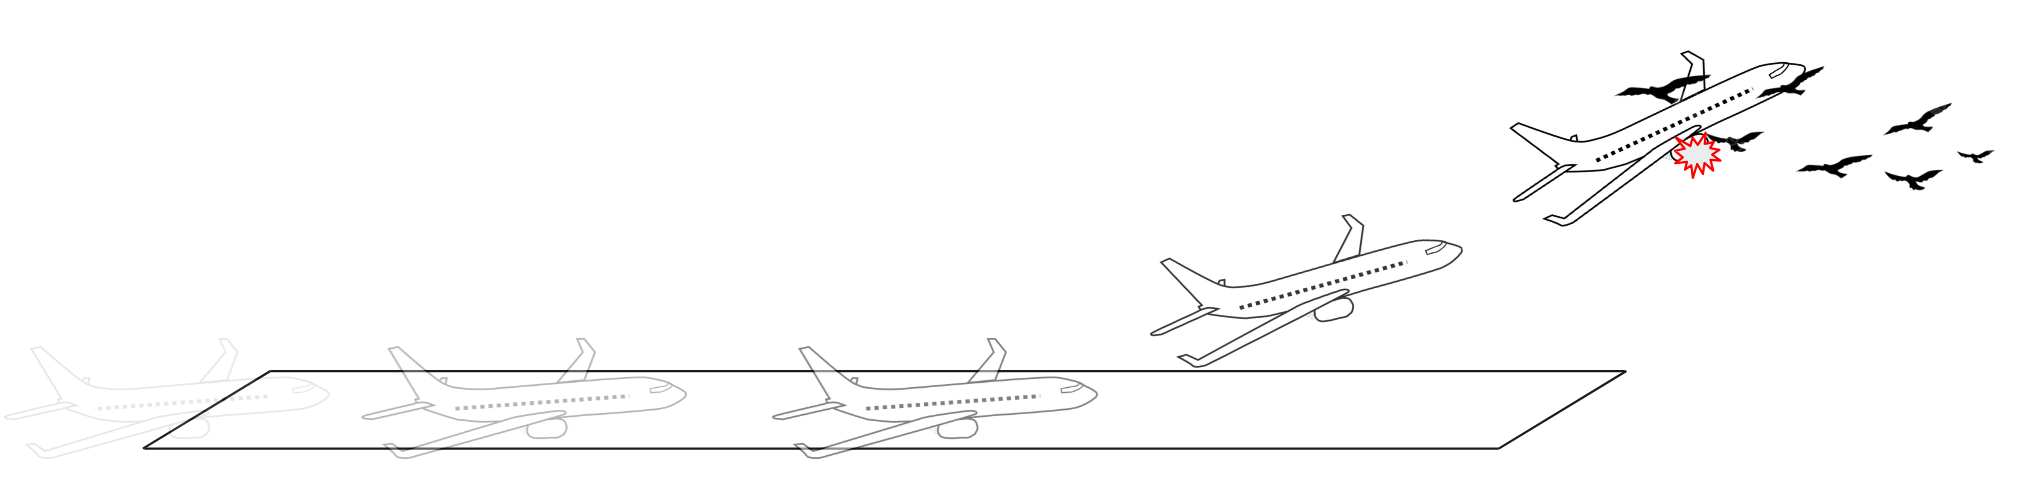
\includegraphics[width=1\textwidth]{./images/scenario.png}
   		\caption{Takeoff scenario with a birdstrike causing an engine failure.}
		\label{fig:takeoff-scenario-simplified}
	\end{figure}

	\subsection{Phase 1: Operational Design Domain analysis}
	The first step of the methodology involves analyzing the current state of commercial aviation operations to understand the scope of the to-be-designed Autonomous Agent (AA) in our operational scenario. Two complementary methods were used for that objective: the Goal Directed Task Analysis (GDTA), and the Interdependence Analysis (IA).

	\subsubsection{Goal-Directed Task Analysis}
	A GDTA was conducted to understand the information needs inherent to commercial aviation operations. GDTA is a task analysis methodology aimed at identifying the critical information human operators must acquire and process to achieve their mission goals effectively and safely.
	Following the established GDTA outlined by \textcite{endsley_designing_2003} for a complete commercial aviation flight, our GDTA was constructed by selecting the relevant hierarchy of goals and associated information requirements for our takeoff scenario. To enrich and validate the GDTA, four experienced commercial pilots were recruited and interviewed. Their insights were incorporated to ensure that the analysis reflects the operational realities of contemporary flight environments.

	The GDTA resulted in a hierarchically organized representation of pilot goals see Figure~\ref{fig:goal-hierarchy}, each associated with the specific information necessary for optimal task performance see Figure~\ref{fig:info_req}. This structured output serves as a foundation for designing the human-autonomy team. Specifically, the identified information elements will guide the development of the Autonomous Agent, ensuring that both the human pilot and the synthetic teammate maintain a sufficient level of SA throughout the operation. The GDTA answers the EASA \textbf{Objective CO-02: for each end user, identify goals and associated high-level tasks that are intended to be performed in interaction with the AA and Objective CO-05: document how end users' inputs are collected and accounted for in the development of the AA} (the complete results of the GDTA can be found in Appendix~\ref{appendix:GDTA}).

	\begin{figure}[H]
		\centering
		\begin{minipage}[b]{1\textwidth}
			\centering
			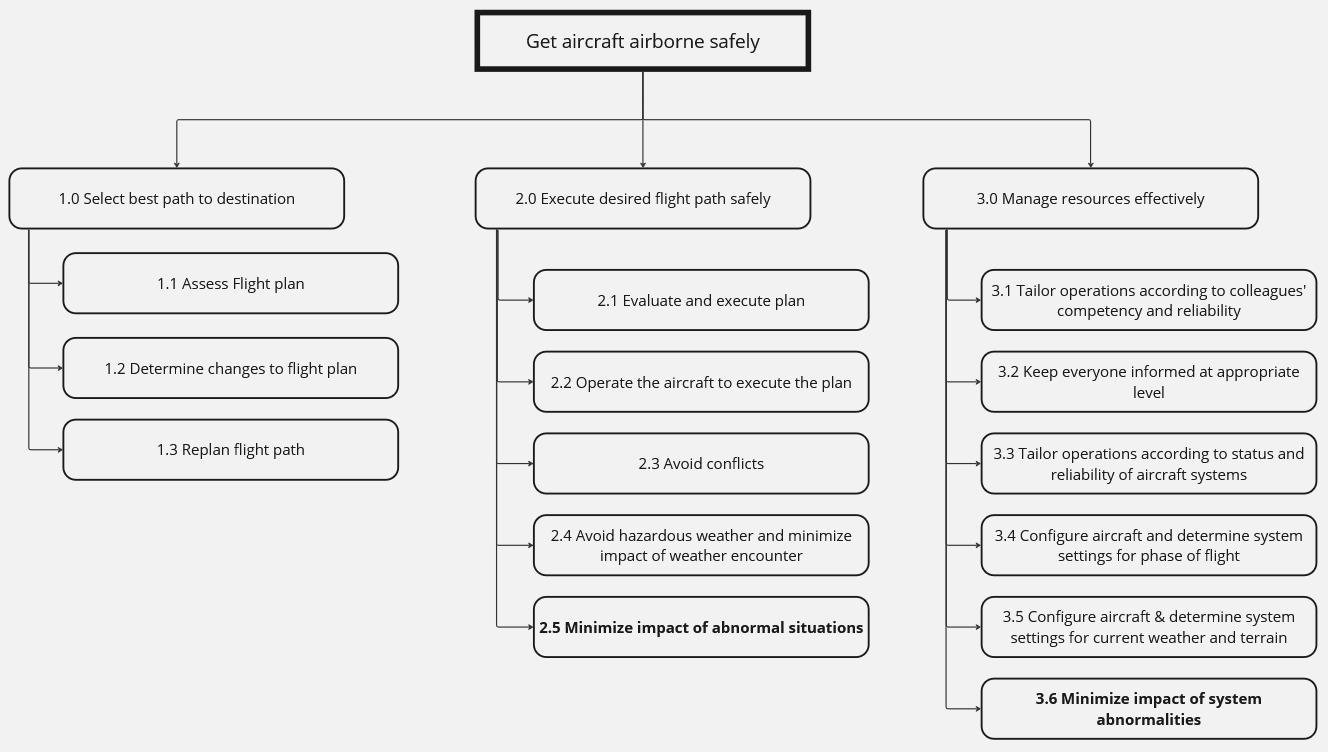
\includegraphics[width=1\textwidth]{./images/gdta_goal_hierarchy.jpg}
			\caption{High-level goal hierarchy}
			\label{fig:goal-hierarchy}
		\end{minipage}
		\begin{minipage}[b]{1\textwidth}
			\centering
			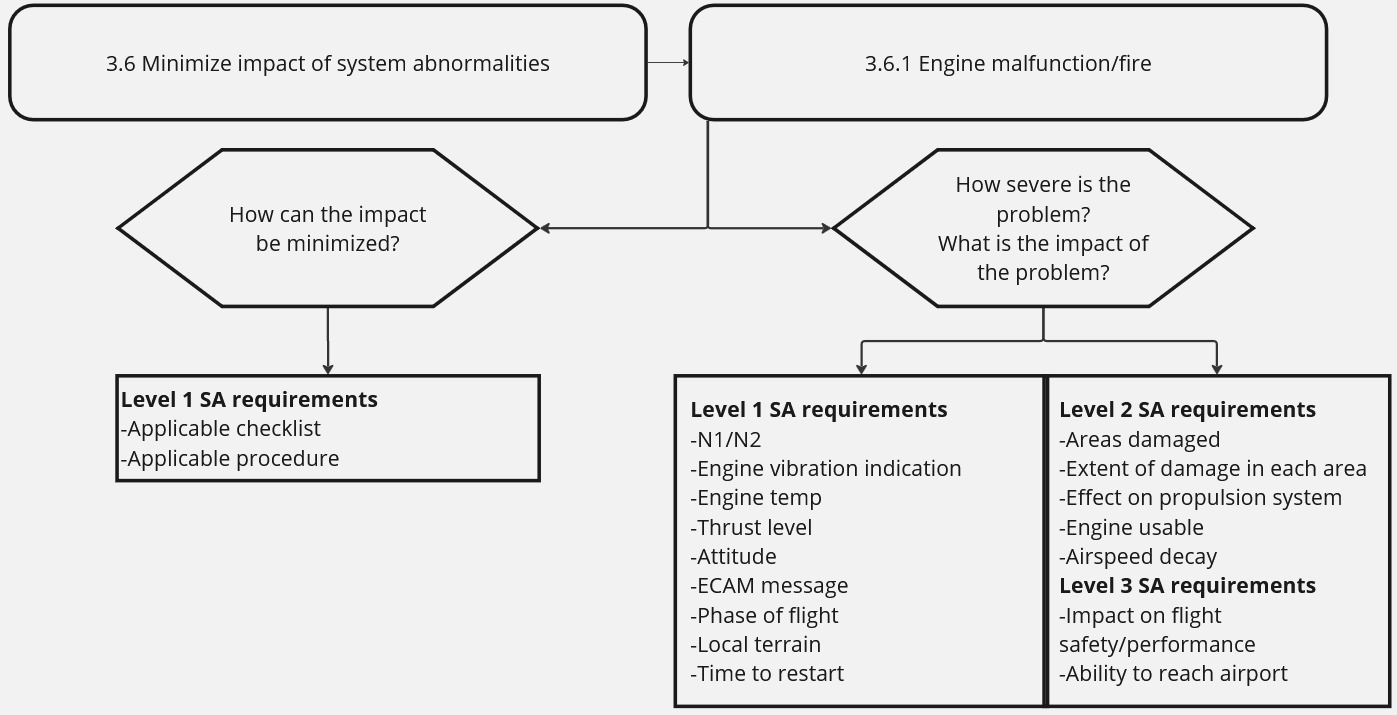
\includegraphics[width=1\textwidth]{images/goal_and_info_req.jpg}
			\caption{Information requirements for goal \textit{3.6.1 - Engine malfunction/fire}}
			\label{fig:info_req}
		\end{minipage}
	\end{figure}

	The goal is to ensure that the human-agent team maintains alignment of their respective situation representation by attending both to the proper information for the task at hand (for example of information requirement see Figure~\ref{fig:info_req}). This alignment supports the development of Team Situation Awareness (Team SA)—the state in which each teammate possesses an accurate understanding of the situation relevant to their roles within the flight deck.
	This notion is visually represented by Figure~\ref{fig:team-sa-venn}, where individual SA of each team member contributes to the larger construct of Team SA. Furthermore, a significant overlap in individual SA defines the concept of Shared Situation Awareness. Achieving and maintaining both individual SA and shared SA between the human and autonomous teammate is critical to ensuring coordinated, safe, and effective operations.

	\begin{figure}[h!]
		\centering
		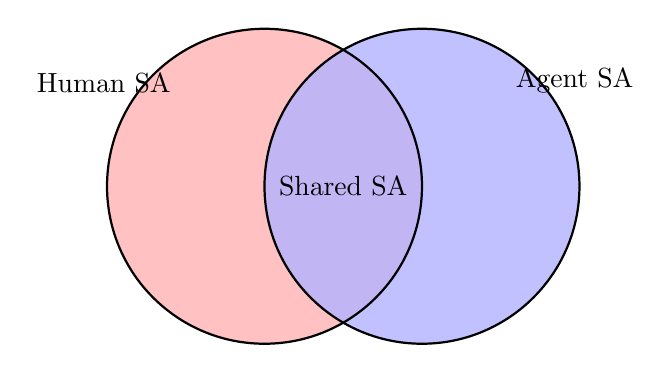
\begin{tikzpicture}
        % Left circle (Human SA)
        \fill[red!30, opacity=0.8] (-1,0) circle (2);
        % Right circle (Agent SA)
        \fill[blue!30, opacity=0.8] (1,0) circle (2);

        % Borders
        \draw[thick] (-1,0) circle (2) node[above left=1.5cm] {Human SA};
        \draw[thick] (1,0) circle (2) node[above right=1.5cm] {Agent SA};

        % Label overlap
        \node at (0,0) {Shared SA};
		\end{tikzpicture}
		\caption{Venn diagram illustrating Team Situation Awareness (Team SA) with the overlapping individual SA of the human pilot and the autonomous agent representing Shared SA.}
		\label{fig:team-sa-venn}
	\end{figure}

	\subsubsection{Interdependence Analysis}
	Interdependent Analysis is a work analysis method part of the coactive design process that helps improve collaboration between humans and machines by identifying key interdependence relationships that are essential for effective teamwork \parencite{johnson_coactive_2014}. It also defines requirements for tasks that involve interdependence, ensuring successful cooperation. 
	
	This framework consists of three main parts: (1) joint activity modeling, (2) interdependence assessment, and (3) workflow analysis. These components help guide the design of systems for more effective teamwork, particularly in human-autonomy teams \parencite{johnson_understanding_2018}.
	
	To define human and autonomy role for our case study we have performed an Interdependence Analysis. This tool's most powerful feature is its ability to map different teaming options at the beginning of the design process, as opposed to a single function allocation solution. The output of an IA gives:
	\begin{itemize}
		\item a sequential hierarchical breakdown of tasks and capacities required to perform the scenario (section 1 of Table~\ref{table:IA}).
		\item Different teaming alternatives, especially in our case, human as main performer of the activity and agent as supporter or agent as the main performer and human as the supporter (section 2 of Table~\ref{table:IA}).
		\item A visualization of possible workflows for the team to carry-out the activity, depending on the team alternative, required, and opportunistic interdependence relationship (section 3 of Table~\ref{table:IA}).
		\item A list of \textbf{Observability, Predictability, and Directability} requirements for each interdependence relations to ensure proper collaboration (Table~\ref{table:OPD}).
	\end{itemize}

	The output of the GDTA was used to facilitates the IA, the goal hierarchy served to create the Joint Activity Graph, which is a hierarchical task decomposition of the activity, and the information requirements also guided the fine-level task definition. 
	
	The Interdependence Analysis answers \textbf{EASA Objective CO-04 - defines and documents the ConOps for the AA, including the possible task allocation pattern between the end user and the AA; Objective CO-06 - perform a functional analysis of the system, as well as a functional decomposition and allocation down to the lowest level} (the full IA table is in Appendix~\ref{table:all-IA}).
	
	\begin{table}[H]
		\centering
		\caption{Interdependence Analysis table excerpt, see Table~\ref{table:color-key} for color key details}
		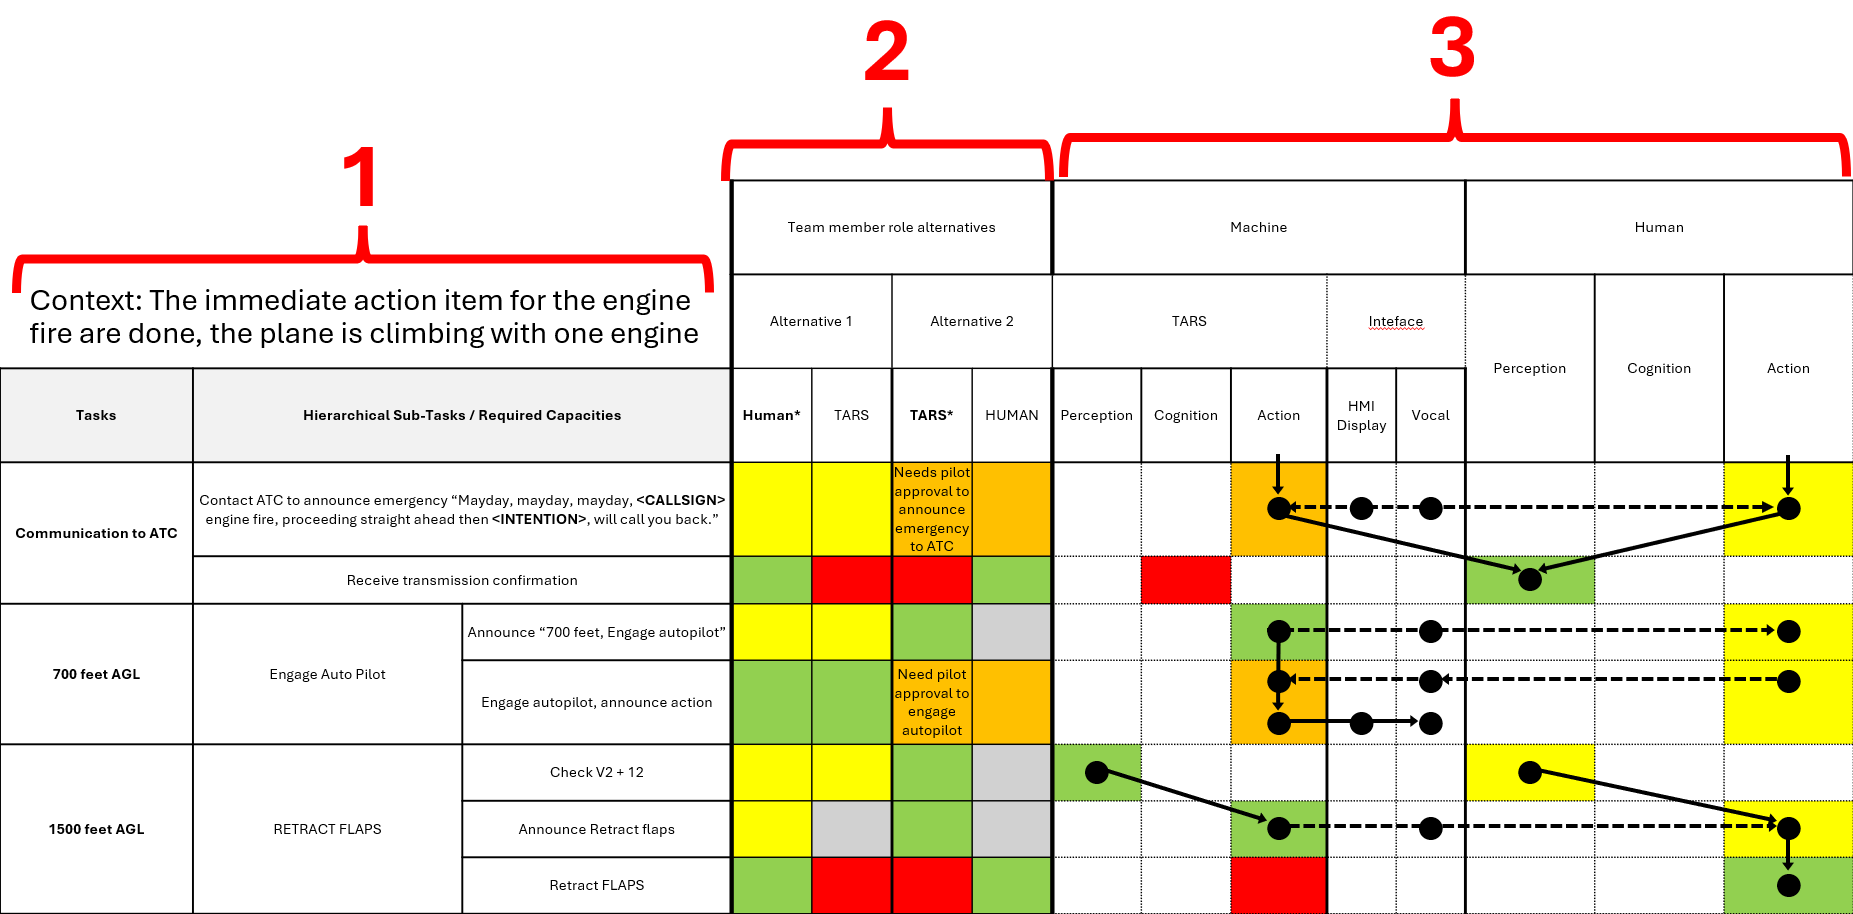
\includegraphics[width=1\textwidth]{images/IA-table.png}
		\label{table:IA}
	\end{table}

	\begin{table}[H]
		\centering
		\caption{Observability, Predictability, Directability requirements excerpt}
		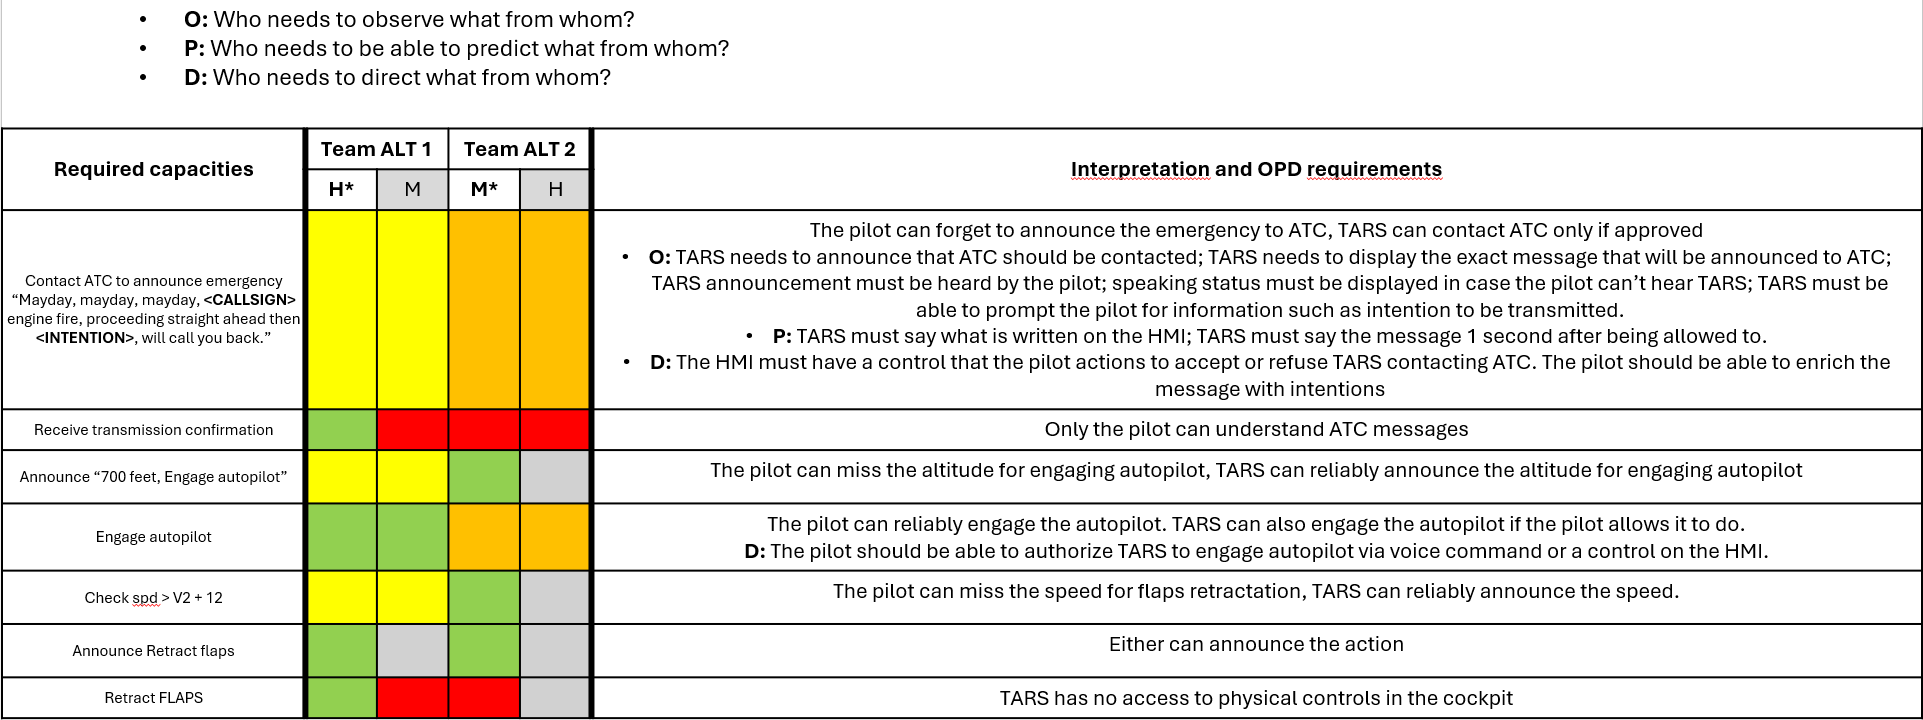
\includegraphics[width=1\textwidth]{images/OPD_table.png}
		\label{table:OPD}
	\end{table}

	The phase 1 and objectives~\ref{obj:1a} and~\ref{obj:1b} have been completed. A chapter titled \textit{"All hands on deck: Case study for Human-Autonomy Teaming (HAT) for Future Commercial Aviation Concepts of Operations"} in the \textit{Handbook of Socio-Technical Systems -- A Human Systems Integration Approach} has been submitted detailing the use-case scenario and methodological approach, it is currently being reviewed.

	\subsection{Phase 2: Cognitive modeling and agent development}

	\begin{figure}[H]
		\centering
		% First logo
		\begin{minipage}[b]{0.3\textwidth}
			\centering
			\raisebox{2mm}{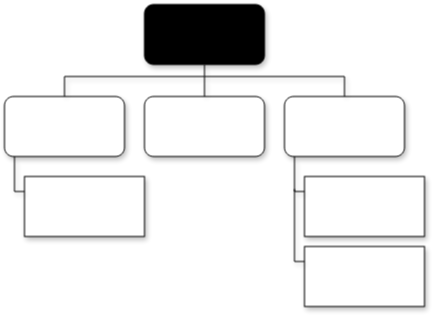
\includegraphics[width=0.9\textwidth]{images/hierarchy_diagram.png}}
		\end{minipage}
		% Second logo
		\begin{minipage}[b]{0.3\textwidth}
			\centering
			
\includegraphics[width=0.6\textwidth]{images/workflow_icon.png}
		\end{minipage}
		% Third logo
		\begin{minipage}[b]{0.3\textwidth}
			\centering
			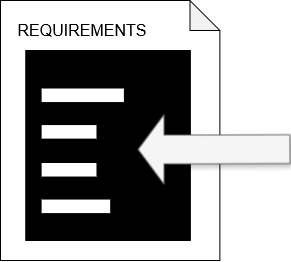
\includegraphics[width=0.8\textwidth]{images/requirements.png}
		\end{minipage}
		\caption{Output of phase 1 - goal hierarchy, task workflow, information \& OPD requirements.}
		\label{fig:logos}
	\end{figure}

	The phase 1 allowed us to list information as well as teaming requirements that will be useful for the modelling and agent design phase, especially:

	\begin{itemize}
		\item The goal hierarchy will be used for the task structure of the cognitive model and the agent, each goal from the GDTA will be implemented in the cognitive model using the goal module of the ACT-R architecture, responsible for holding the current goal or focus of attention of the model. Likewise, agent-side, the goal hierarchy will be represented as a structure containing states and transitions akin to a Finite State Machine (FSM)
		\item Workflows from the IA will be used as an input to a module responsible for the task allocation between the model and the agent, for each workflow, this "dispatcher" module will effectively activate or inhibit actions for the model and agent.
		\item Information requirements will be used to program that both the model and agent attend to the relevant elements of the environment for the task at hand. It will also be used for SA assessment, as the cognitive model can be asked to answer questions regarding the value/status of relevant information for the task, and information representation of the AA can be inspected at any time, thus the alignment in SA can be approximated by the difference in situation representation for both teammates. OPD requirements will be individually assessed during simulation and experiments by observing team behavior.
	\end{itemize}

	\subsubsection{QN-ACTR and SEEV}
	\label{qn-actr-seev}
	The cognitive model of the single pilot will be implemented using the QN-ACTR architecture, integrating a SEEV model to capture attention allocation dynamics and level 1 situation awareness (SA). Based on the output from Phase 1, operational documentation, and available training materials, an initial model of an expert pilot takekoff will be developed. The model will simulate routine procedural execution, following Standard Operating Procedures (SOPs) and checklists for the aircraft type \textbf{without any assistance from an autonomous agent} (baseline model).

	The model will be connected to X-Plane 11 in a closed-loop simulation, receiving real-time aircraft and environment data and issuing control inputs directly to the simulator via UDP. Once the baseline model can effectively navigate the scenario, it will be extended to collaborate with the autonomous agent, enabling it to observe and direct the agent's actions.
	
	The model ACT-R lisp model will be integrated into the QN-ACTR platform, with necessary adjustments to ensure appropriate input/output handling with X-Plane 11. Development will build upon the QN-ACTR takeoff model by \textcite{xu_modeling_2021}, which currently models a single-pilot normal takeoff procedure in a Cessna 172 aircraft.
	
	The SEEV module will be applied to determine the probability of the model allocating attention to relevant Areas of Interest (AOIs) in the cockpit and external environment. The SEEV parameters—Salience, Effort, Expectancy, and Value—will initially adopt the coefficient weights proposed by \textcite{wang_real-time_2024}, whose model was tuned for a similar scenario (engine failure at takeoff in Single Pilot Operations). Their configuration defines seven AOIs: (1) Primary Flight Display (PFD), (2) Navigation Display (ND), (3) Engine/Warning Display (E/WD), (4) System Display (SD), (5) Central Console, (6) Flight Manual, and (7) Outside Window. Equation~\ref{eq:VA_AOI} details the SEEV module.
	
	\begin{equation}
		VA_{AOI} = \sum_{t=1}^{n} (Ex_t) (R_t) (P_t)
		\label{eq:VA_AOI}
	\end{equation}
	Here, $VA_{AOI}$ is the raw attention value for an AOI, $t$ indexes across $n$ tasks, $Ex_t$ is the Expectancy of the AOI for task $t$, $R_t$ is its Relevance, and $P_t$ is the Priority of task $t$. The combined effect of $R_t$ and $P_t$ represents the "Value" factor in the SEEV model.
	
	The resulting $VA_{AOI}$ values are normalized to generate probabilistic attention weights across all AOIs. Monte Carlo simulations will be used to stochastically determine gaze allocation over time.
	
	The model accounts for both attentional and memory constraints: attention allocation drives what information enters the cognitive system, while ACT-R's declarative memory mechanisms (e.g., memory decay and activation thresholds) govern subsequent retention and retrieval. In QN-ACTR, activation levels of chunks representing critical elements must exceed a threshold to contribute to Level 1 SA (perception-based SA). Consequently, Level 1 SA in this model emerges from the interaction between visual attention (SEEV) and cognitive memory dynamics (ACT-R). The framework is presented in Figure~\ref{fig:qn-actr-seev}

	\begin{figure}[H]
    \centering
    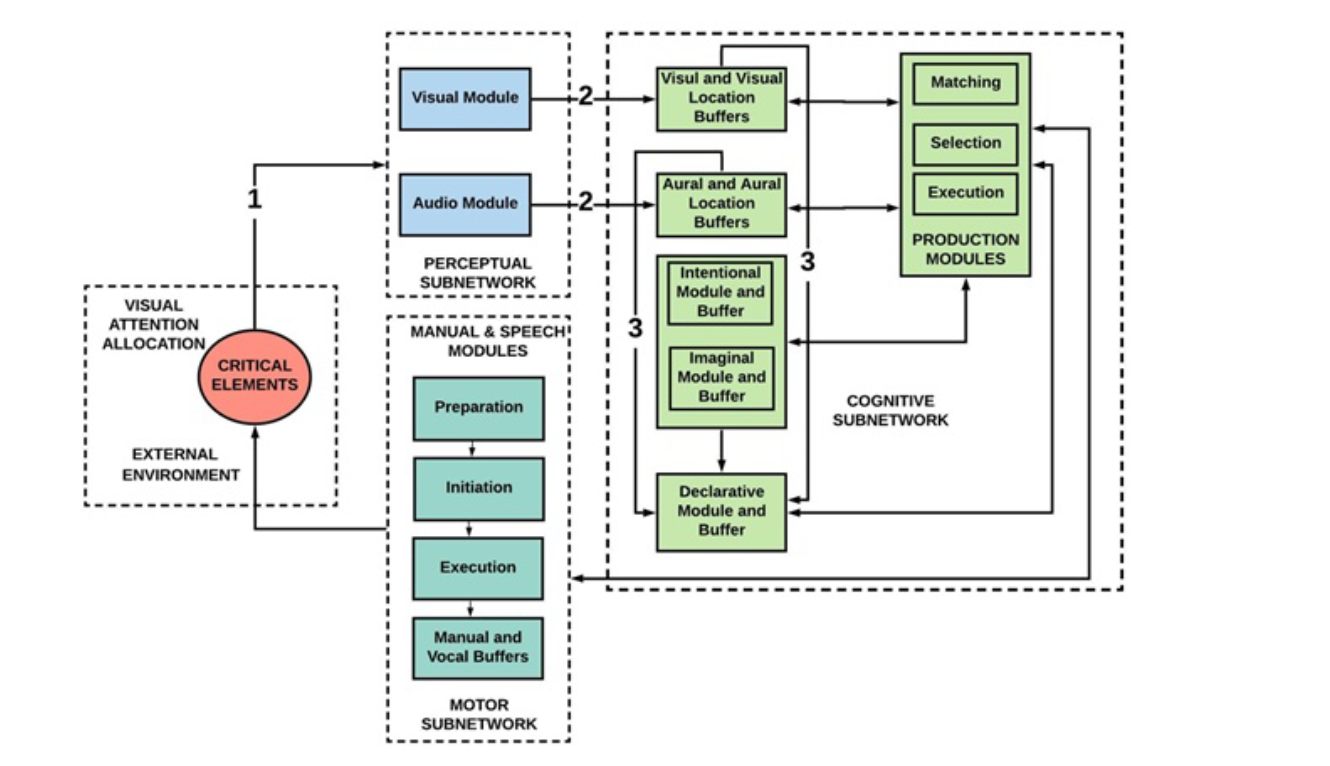
\includegraphics[width=0.9\textwidth]{./images/qn-actr-sa-synoptic.png}
    \caption{Overview of the QN-ACTR-SEEV framework. Stages 1-3 (marked on the lines in the figure) signify the different cognitive processes necessary in the acquisition and maintenance of Level 1 SA. Adapted from Rehman (2020) \parencite{rehman_phd_thesis}.}
    \label{fig:qn-actr-seev}
	\end{figure}

	\subsubsection{Agent design}
	A functional prototype of the Autonomous Agent (AA) system will be developed in parallel with the cognitive model to meet the previously defined requirements. The prototype will be deployed as a tablet application interfacing with the flight simulator and positioned within the cockpit environment.

	The AA is implemented as a modular and reactive software component designed to assist the pilot in managing the flight scenario.
	\paragraph{Objective CO-03 - Definition of the AA system:} The agent adopts a nested Finite State Machine (FSM) architecture, employing the state pattern, to organize its behavior into a structured hierarchy of states and substates. Each state encapsulates a specific procedural phase of the scenario, with transitions triggered by defined environmental conditions.
	
	This design was selected to reflect the deterministic and highly procedural characteristics of the flight scenario chosen. The agent does not incorporate deliberative planning or uncertainty handling; rather, it functions as a partial Wizard of Oz system. Its purpose is to emulate the expert-like behavior of an AI system that executes preprogrammed actions in response to parameters perceived in the simulation environment.
	
	The AA system is composed of the following modules: 
	\begin{itemize} 
		\item \textbf{State Hierarchy:} A layered structure of states and nested substates representing sequential and conditional phases of the flight (e.g., "Takeoff Roll" $\rightarrow$ "Engine-Out Emergency Procedure" $\rightarrow$ "Communicate with ATC").
		\item \textbf{State Manager:} A supervisory module responsible for managing transitions between states based on predefined transition rules.
		\item \textbf{Action Layer:} A set of atomic actions (e.g., "Verify engine instruments", "Declare emergency to ATC") executed when specific states or substates become active.
		\item \textbf{Status Monitoring:} A continuous input channel from the flight simulator (X-Plane 11) used to assess scenario conditions and update the agent's internal state. 
		\item \textbf{Cockpit AA Interface:} A graphical and/or auditory interface that communicates the agent's current state, intended actions, and contextual information to the pilot. It is designed to support real-time awareness by providing timely and relevant cues aligned with the scenario's procedural flow.
	\end{itemize}
	\paragraph{Objective HF-01 - design the AA with the ability to build its own individual situation representation:}
	The agent maintains an implicit representation of the current situation by continuously monitoring the flight environment and updating its active state within the nested FSM hierarchy. This evolving internal state reflects the agent's interpretation of procedural phases and contextual conditions. Although the system does not engage in deliberative reasoning or planning, this structured state-driven representation allows the AA to maintain an internal situation model akin to human SA.
	\paragraph{Objective HF-02 - Reinforcing Pilot Situation Awareness; Objective HF-03 - Support shared situation awareness:}  
	To support the pilot's situation awareness, the AA system incorporates a dedicated cockpit interface that provides transparent access to its current state and behavioral intent. By externalizing the agent's internal state transitions and highlighting critical contextual information (e.g., detected anomalies, pending actions, communication cues), the interface reinforces the pilot's understanding of the evolving scenario. 

	In conclusion, the nested FSM structure provides a modular and scalable framework, ensuring ease of maintenance and facilitating the alignment between the agent's reactive behavior and the cognitive model's.

	\begin{figure}[H]
		\centering
		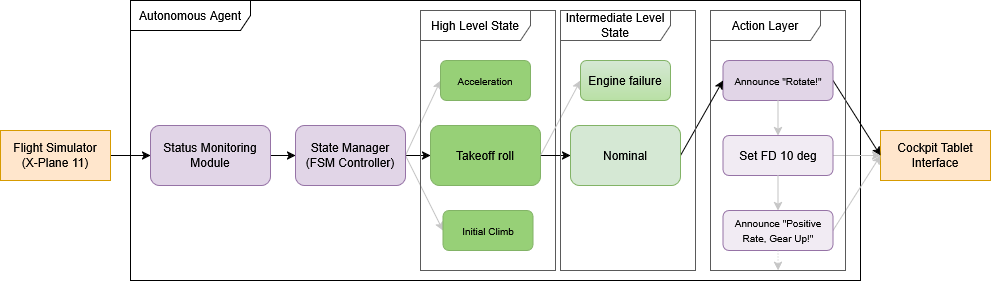
\includegraphics[width=1.0\textwidth]{./images/AA_synoptic.png}
		\caption{AA Synoptic diagram}
		\label{fig:aa_synoptic}
	\end{figure}
	
	\subsubsection{System architecture}
	The complete system architecture consists of five principal components: the Cognitive Model (QN-ACTR + SEEV), the Autonomous Agent (AA), the Task Dispatcher, the Aircraft and Environment (X-Plane 11), and the Human-AA Interface. These components operate within the same local network and interact in real time to simulate a functional Human-Autonomy Teaming (HAT) environment.
	
	\begin{itemize} 
		\item \textbf{Task Dispatcher:} A central module responsible for allocating tasks between the cognitive model and the AA. The dispatcher can be thought of as representing the Human-Autonomy orchestrator. It activates or inhibits tasks for each member of the team, ensuring overall coherence between entities for effective collaboration to achieve the shared set of goals. It also automates simulation batches.
		
		\item \textbf{Cognitive Model:} The QN-ACTR+SEEV model simulates the pilot's cognitive processes, including level 1 situation awareness. It is capable of both executing tasks directly on X-Plane and interacting with the AA.
	
		\item \textbf{Autonomous Agent (AA):} Handles delegated tasks from the dispatcher and takes direct action in the simulation environment to assist the pilot.
	
		\item \textbf{Aircraft and Environment (X-Plane 11):} The simulation environment provides the dynamic flight scenario, including aircraft behavior and environmental conditions. It represents the shared operational context in which both the AA and the cognitive model are embedded.
	
		\item \textbf{Human-AA Interface:} A tablet-based application implemented as a dedicated interface between the human pilot and the AA system. It enables the agent to externalize its internal state and communicate intentions, actions, and context-sensitive information, reinforcing shared situation awareness and facilitating coordination within the HAT.
	\end{itemize}
	
	The system leverages the \textbf{Ingescape ecosystem} to connect distributed modules seamlessly:
	\begin{itemize}
		\item \textbf{Black-box agents:} Each software module (dispatcher, cognitive model, AA agent) is implemented as an independent black box with defined input/output ports.
	
		\item \textbf{ZeroMQ-based messaging:} Ingescape abstracts communication, enabling asynchronous and decoupled messaging between components.
	
		\item \textbf{Simulation Interface:} The AA and cognitive model both exchange real-time data with the X-Plane 11 environment and with each other, ensuring synchronized and coherent situational representations across components. The Human-AA Interface also receives updates from the AA agent to inform the pilot in real time.
	\end{itemize}
	
	This modular and distributed architecture enables flexible experimentation with various teaming strategies, and supports incremental development or substitution of individual system components, see Figure~\ref{fig:ingescape_platform}.
	
	\begin{figure}[H] 
		\centering
		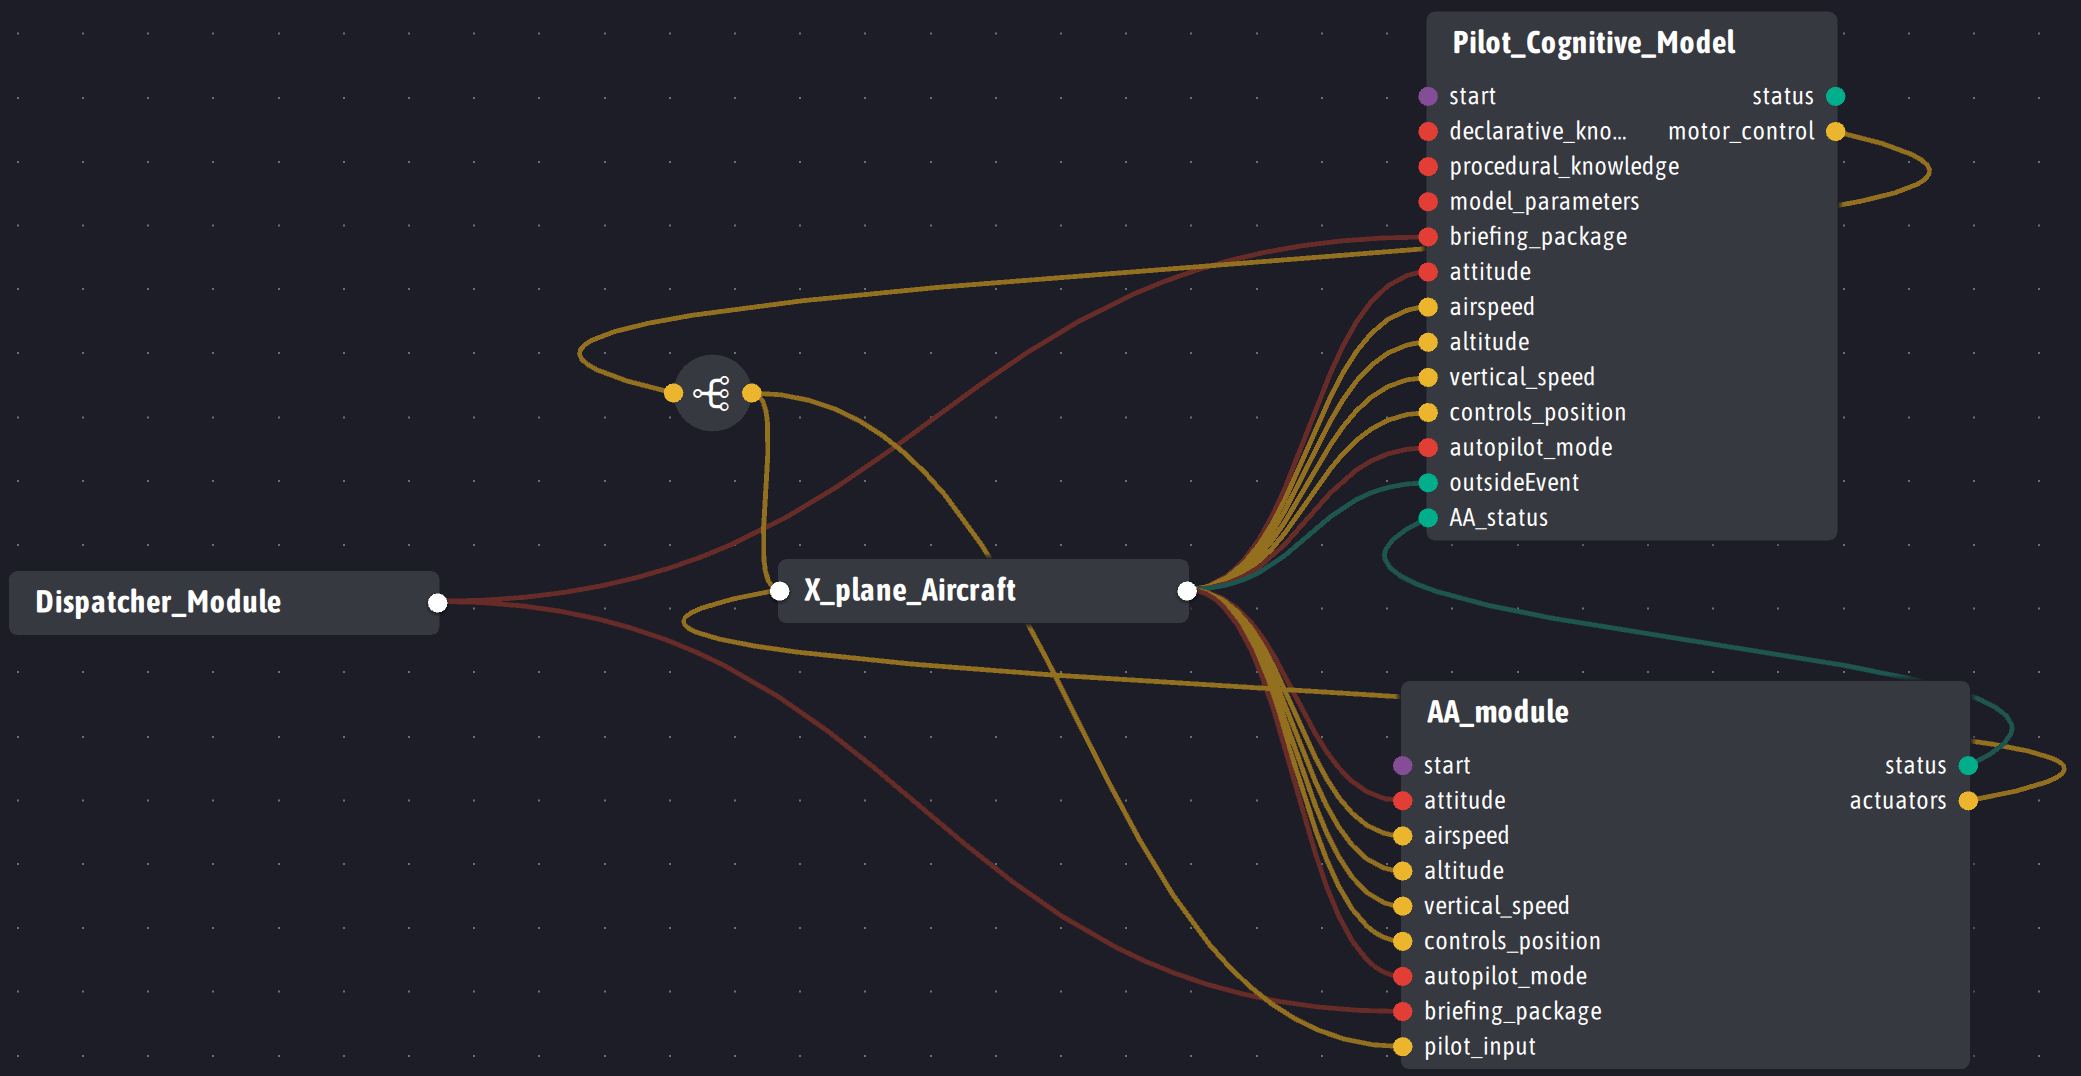
\includegraphics[width=1.0\textwidth]{./images/ingescape_platform.png}
		\caption{System architecture overview from the Ingescape platform}
		\label{fig:ingescape_platform}
	\end{figure}
	

	\subsubsection{Scenario \& Simulation}
	We constructed the scenario based on checklists, standard operating procedures (SOPs), training material, and feedback from subject matter experts of the Cessna Citation Mustang. This aircraft is single-pilot certified, meaning that the required procedures are currently performed by either a single pilot or a two-pilot crew. This aspect eased the construction of the cognitive model, because a baseline single-pilot operation (SPO) already exists, eliminating the need to invent new procedures. We ensured that our scenario remains as close to operational reality as possible, it is depicted in~\ref{fig:scenario_detailed}.

	\begin{figure}[H]
		\centering
		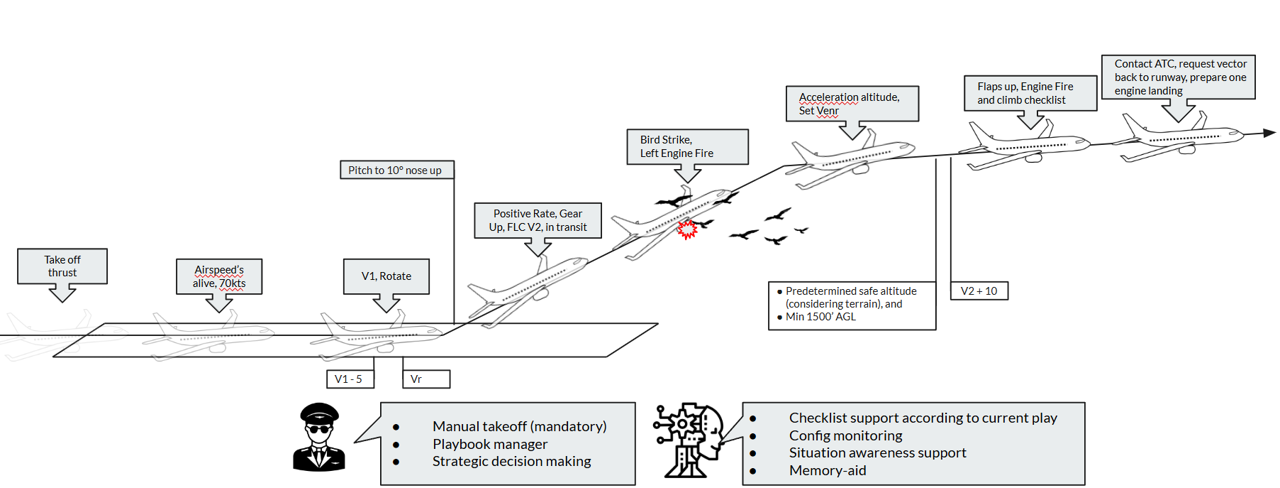
\includegraphics[width=1.0\textwidth]{./images/scenario_detailed.png}
		\caption{Takeoff scenario detailed}
		\label{fig:scenario_detailed}
	\end{figure}

	Upon completing the development of both the cognitive model and the autonomous agent, we will enter the simulation phase to gather data. The experiment will involve two independent variables, each designed to examine different aspects of human-autonomy teaming in aviation represented by 5 different dependent variables, all synthesized in Table~\ref{tab:variables}.
	
	\textbf{Independent Variables}
	The primary goal of this research is not to determine the optimal Human-AI teaming configuration, but rather to demonstrate that a cognitively plausible model of Situation Awareness (SA) can be used to systematically evaluate and compare different Human-Autonomy Teaming (HAT) configurations. The experimental design therefore aims to test the viability of the proposed methodology across conceptually distinct types of HAT relationships, rather than optimize for operational performance.

	\begin{itemize}
	\item \textbf{IV1: Teaming Mode (Task Allocation Strategy)}
	This variable corresponds directly to the EASA HAT taxonomy level, and allows comparison between fundamentally different Human-AI interaction paradigms:

	\begin{itemize}
	\item \textbf{No teaming (single pilot without AA) - Baseline condition}
	\item \textbf{Fixed Task Allocation (Cooperation – Level 2A)}:  
	The task allocation between the human pilot and the Autonomous Agent (AA) is defined during the pre-flight briefing and remains fixed throughout the scenario. The AA acts as a supporting agent and does not adapt its behavior based on unfolding events beyond what is pre-programmed.

	\item \textbf{Dynamic Task Allocation (Collaboration – Level 2B)}:  
	The pilot may dynamically reassign tasks to the AA during the scenario using a "playbook"-style interface. This mode supports runtime task reallocation in response to non-nominal events.
	\end{itemize}

	\item \textbf{IV2: Scenario Condition}
	This variable introduces operational complexity and assesses how each teaming mode performs under different environmental demands.

	\begin{itemize}
	\item \textbf{Nominal Condition}:  
	Standard takeoff without any anomalies.
	\item \textbf{Non-Nominal Conditions - Engine Failure in Flight}: Bird strike and engine failure after V1.
	\end{itemize}
	\end{itemize}

	This 2x3 design allows us to test whether the proposed methodology can capture meaningful differences in performance, workload, and situation awareness across three representative HAT configurations and operational challenges. The chosen teaming modes are deliberately distinct to maximize conceptual coverage (no teaming vs Cooperation vs Collaboration) rather than incrementally vary one design variable (e.g., more or less reliable path predicted by the interdependence analysis). By validating the cognitive model against both configurations, we aim to establish the feasibility and generalizability of the approach for future design evaluation of AI teammates in aviation.

	\textbf{Dependent Variables}
	\begin{itemize}
		\item \textbf{DV1 : Situation Awareness (SA) / Situation Representation}:
		\begin{itemize}
			\item Assessed through the SAGAT (Situation Awareness Global Assessment Technique) methodology at various points in the scenario.
			SAGAT questions are derived from the GDTA (Goal-Directed Task Analysis) information requirements and will be probed to the cognitive model by pausing the simulation at predefined moments.
			\item The autonomous agent's current situation representation will be retrieved simultaneously by inspecting relevant flight parameters values as defined by the information requirements.
		\end{itemize}
		\item \textbf{DV2 : Workload}:
		\begin{itemize}
			\item Estimated workload levels are automatically output by QN-ACTR. The architecture considers ACT-R modules and buffers as servers and uses "Expected Utilization as a workload index to capture the impact of time stress. Expected Utilization is defined as the ratio of the server processing time required by task demands to the total available task time" \parencite{cao_modelling_2015}.
			\begin{equation}
				Expected\ Utilization = \frac{Time_{required}}{Time_{total}} 
			\end{equation}
			Workload is assumed to have a linear relationship with the overall expected utilisation (OEU) averaged from all servers that have non-zero service time
		\end{itemize}
		\item \textbf{DV3 : Performance Metrics}:
		\begin{itemize}
			\item Time to return to a nominal flight condition following the bird strike: Time to execute the emergency procedures and checklist.
		\end{itemize}
		\item \textbf{DV4 : Attention Allocation and Gaze Behavior}:
		\begin{itemize}
			\item The cognitive model's gaze patterns and attention allocation toward Areas of Interest (AoIs) will be analyzed, including fixation count and total gaze time per AoI.
		\end{itemize}
		\item \textbf{DV5 : Teaming Effectiveness Evaluation}:
		\begin{itemize}
			\item Systematic validation of teaming requirements (except Predictability which would require modelling of anticipation --- SA level 3 --- which is outside of the scope of this thesis), this also corresponds to EASA \textbf{Objective LM-10 - perform requirements-based verification of the trained model behaviour}:
		\end{itemize}
	\end{itemize}
	
	\textbf{Simulation Repetitions and Statistical Analysis}
	Given the stochastic nature of the cognitive model's attention allocation module, each condition will be repeated the same number of times than participants recruited for HITLS.

	\textbf{Hypotheses :}
	\begin{enumerate}[label=\textbf{H\arabic* :}]
	\label{hypotheses}
	\item \textbf{Workload predicted level}: No teaming $>$ 2B - Collaboration $>$ 2A - Cooperation
	\item \textbf{Situation Awareness level}: No teaming $<$ 2A - Cooperation $\approx$ 2B - Collaboration (no significant differences between teaming configurations)
	\item \textbf{Team SA alignment}: 2A - Cooperation $<$ 2B - Collaboration. Which means that in collaboration, the cognitive model's critical information representation's value should closely match the autonomous agent's
	\item \textbf{Performance level}: No teaming $<$ 2A - Cooperation $\approx$ 2B - Collaboration
	\item \textbf{Fixation count and gaze time on the autonomy's HMI}: 2A - Cooperation $<$ 2B - Collaboration
	\end{enumerate}
	Additionally, we anticipate being able to systematically validate the \textbf{Observability} and \textbf{Directability} requirements during the simulation phase.
	
	\begin{table}[h]
		\centering
		\caption{Independent and Dependent Variables Overview}
		\renewcommand{\arraystretch}{1.3}
		\resizebox{\textwidth}{!}{ % This scales the table to fit within text width
		\begin{tabular}{|l|l|}
			\hline
			\textbf{Independent Variables} & \textbf{Levels} \\
			\hline
			\textbf{Teaming Configuration} & \begin{tabular}[c]{@{}l@{}}Baseline: Cognitive model alone in SPO \\ 2A - cooperation (fixed pre-allocation) \\ 2B - collaboration (re-allocation in real-time)\end{tabular} \\
			\hline
			\textbf{Scenario Variations} & \begin{tabular}[c]{@{}l@{}}Nominal: No bird strike \\ Non-Nominal: \\ - Bird strike + engine failure after V1\end{tabular} \\
			\hline
			\textbf{Dependent Variables} & \textbf{Measurement Approach} \\
			\hline
			\textbf{Situation Awareness (SA)} & \begin{tabular}[c]{@{}l@{}}SAGAT score \\ Agent's situation representation captured simultaneously\end{tabular} \\
			\hline
			\textbf{Cognitive Model Workload} & \begin{tabular}[c]{@{}l@{}}Output from QN-ACTR Expected Utilization\end{tabular} \\
			\hline
			\textbf{Performance Metrics} & \begin{tabular}[c]{@{}l@{}}Engine failure after takeoff: Time for completing emergency procedures\end{tabular} \\
			\hline
			\textbf{Attention Allocation and Gaze Behavior} & \begin{tabular}[c]{@{}l@{}} Fixation count and gaze time on Autonomous agent's HMI\end{tabular} \\
			\hline
			\textbf{Teaming Effectiveness Evaluation} & \begin{tabular}[c]{@{}l@{}}Validation of teaming requirements: \\ - Observability: Agent's actions must be observable \\ - Directability: Pilot must be able to direct the agent\end{tabular} \\
			\hline
		\end{tabular}
		}
		\label{tab:variables}
	\end{table}

	The phase 2 will complete objectives~\ref{obj:2a}, \ref{obj:2b}, \ref{obj:2c} and \ref{obj:2d}. We expect to publish a journal article detailing the coupling of a situation awareness cognitive model and an autonomous agent in a closed-loop simulation study, as well as simulation results and how they can be used to iterate the design of the agent and HMI. According to our research, this is a novel contribution, our goal is to publish in a Human-Computer interaction / human factors research journal, preferably an issue on Human Performance Modelling / cognitive modelling.

	\subsection{Phase 3: Human-In-The-loop simulation studies}
	At the end of the phase 2 we should have a cognitive model able to team up with an autonomous agent in a simulated SPO flight providing SA and human performance data. This will allow us to run automated studies evaluating Human-Autonomy Teaming. However, at this stage, \textbf{we do not have any confirmation that the data generated indeed predicts human performance}; our model needs to be validated. This means we need to recruit expert pilots to take part in the same simulated flight as the model to check whether our assumptions about pilot cognition compare with empirical results.

	\subsubsection{Scenario}
	The scenario for the Human-in-the-Loop Simulation (HITLS) study is identical to the one executed by the cognitive model see Figure~\ref{fig:scenario_detailed}. It involves the same aircraft type, cockpit layout, SOPs, route, weather conditions, and emergency procedures to ensure consistency and comparability between computer simulation and human experiments.

	\subsubsection{Equipment}
	The study will be conducted in the full-flight simulator at Polytechnique Figure~\ref{fig:simu_cockpit}A, which represents the cockpit layout of a Beechcraft Baron G58 equipped with Garmin G1000 avionics. This setup is highly similar to the Cessna Citation Mustang's cockpit Figure~\ref{fig:simu_cockpit}B, ensuring minimal differences in interface and procedural interactions. A camera-based eye tracker (spec ??) will be integrated into the simulator to capture gaze behavior, with defined Areas of Interest (AoIs) matching those in the cognitive model's SEEV module (\ref{qn-actr-seev}). Pilot actions, will be recorded using the embedded camera of the simulator's cabin.

	\begin{figure}[H]
		\centering
		% First logo
		\begin{minipage}[b]{0.50\textwidth} % Adjusted width
			\centering
			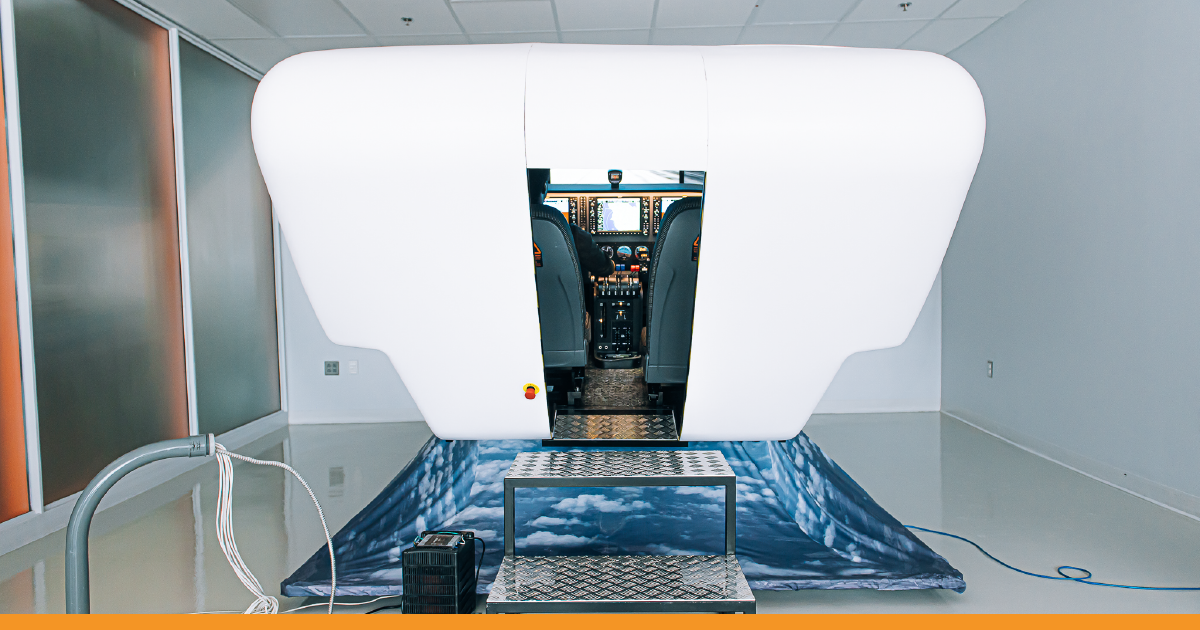
\includegraphics[width=\textwidth]{images/poly_simu.png}
		\end{minipage}
		\hfill % Adds space between the two figures
		% Second logo
		\begin{minipage}[b]{0.45\textwidth} % Adjusted width
			\centering
			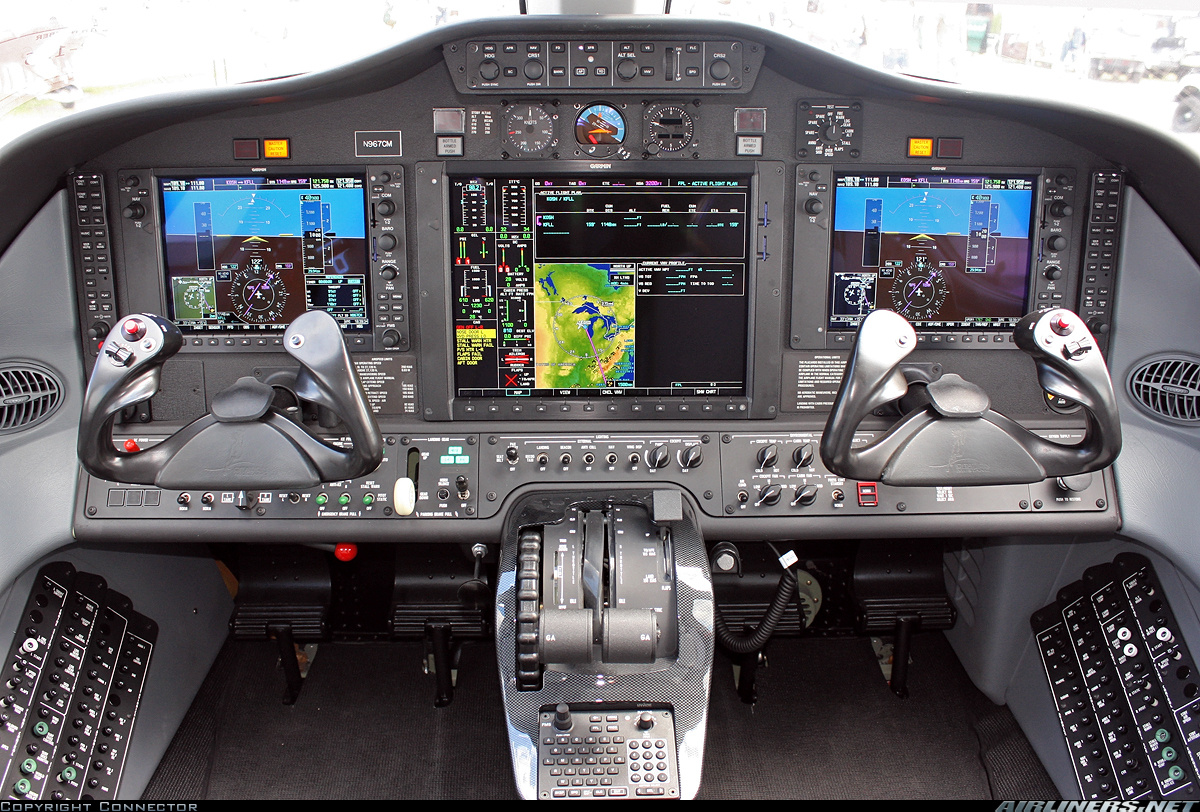
\includegraphics[width=\textwidth]{images/mustang_cockpit.jpg}
		\end{minipage}
		\caption{(A) Polytechnique's simulator and (B) Cessna Citation Mustang cockpit.}
		\label{fig:simu_cockpit}
	\end{figure}
	

	\subsubsection{Participants}
	We will recruit at least 15 pilots holding a Commercial Pilot License (CPL) with prior experience in multi-crew operations. This ensures that participants are familiar with the teamwork dynamics necessary for human-autonomy teaming studies.

	\subsubsection{Protocol}
	Each pilot will undergo a formal pre-flight briefing phase before each scenario. The briefing will adhere to aviation standards, covering:
	\begin{itemize}
		\item Route and weather conditions
		\item Departure and emergency procedures
		\item Communication and automation plans
		\item Human-AI crew roles and task allocation plan
		\item Aircraft performance 
	\end{itemize}
	This briefing phase is crucial, as identified in the GDTA and pilot interviews, participants emphasized that "\textit{The Plan}" established during briefing dictates the crew's actions and cooperation throughout the flight. Pilots only deviate from \textit{The Plan} in unexpected situations, and a bird strike and engine failure at takeoff is considered during the briefing, reinforcing the need for a structured pre-flight preparation.

	Participants will first complete the nominal familiarization scenario. This phase introduces them to Polytechnique's simulator and the autonomous agent's interface, to reduce training effect. Then pilots will be performing the non-nominal scenario 3 times for each teaming configuration, we will counterbalance the order for each participants. 

	During the scenario, the simulator will be paused at predefined moments to administer SAGAT probes assessing the pilot's situation awareness. Pilot's gaze behavior will be continuously recorded.

	Given that Predictability is the only OPD requirement not covered by the cognitive model, special SAGAT probes will be asked to verify if pilots can anticipate the behaviour of the autonomous agent, thus validating this final set of requirements.
	
	Scenarios are less than 10 minutes long.

	After each scenario, pilots will complete the NASA-TLX standardized workload assessment questionnaire and SUS (System Usability Scale) usability questionnaire to evaluate the human-agent interface. After every scenarios, pilots will engage in a semi-structured debriefing interview discussing trust in the autonomous agent, HMI design, future human-autonomous agent crew roles, and any qualitative feedback they might have.

	\subsubsection{Model validation and results}
	The HITLS serves two primary objectives. First, validating the model \ref{obj:3a}, by comparing simulated results with human empirical data, especially:
	\begin{enumerate}
		\item Simulated vs. empirical SAGAT scores.
		\item Simulated workload vs. NASA-TLX scores.
		\item Fixation count and fixation per AoI for both the cognitive model and human pilots.
		\item Compare simulated vs. empirical time to resolve emergencies in non-nominal scenarios. 
	\end{enumerate}
	The same hypotheses (\ref{hypotheses}) as defined during the computer simulation phase will be applied to the HITLS study to assess model fidelity. 

	The model's goodness-of-fit will be assessed using Mean Absolute Percentage Error (MAPE), Root Mean Square Error (RMSE) and Coefficient of determination (R-squared).

	\begin{equation}
		RMSE = \sqrt{\frac{\sum_{i=1}^{n} \left(X_{human,i}-X_{model,i}\right)^2}{n} } 
	\end{equation}

	\begin{equation}
		MAPE = \frac{100}{n} \sum_{i=1}^{n} \left\lvert \frac{X_{human,i} - X_{model,i}}{X_{human,i}} \right\rvert 
	\end{equation}

	\begin{equation}
		R^2 = 1 - \frac{\sum_{i=1}^{n} (X_{human,i} - X_{model,i})^2}{\sum_{i=1}^{n} (X_{human,i} - \bar{X}_{human})^2}
	\end{equation}

	The second objective is to investigate non-modelable human factors \ref{obj:3b}, specifically predictability of autonomous agents's behaviour, trust, and usability aspects. We will also gather qualitative feedback on autonomous agent and HMI design and subjective responses regarding future human-autonomy crew roles.
	
	\section{Originality and Impact}

	This research project introduces an original methodology for evaluating Human-Autonomy Teaming (HAT) in the context of commercial aviation through the use of cognitive modeling. While several papers have outlined the theoretical potential of using cognitive architectures for evaluating human-autonomy collaboration, to date, no full-scale implementation has been conducted. This proposal operationalizes such a framework by embedding a cognitively plausible pilot model within a closed-loop simulation that also includes an autonomous agent, a task dispatcher, and a human-agent interface; all interacting in real-time with a high-fidelity flight simulator.
	
	A key element of originality lies in the use of the QN-ACTR-SEEV cognitive architecture to simulate attention allocation and memory dynamics in aviation, allowing for an objective, model-based assessment of Situation Awareness (SA) and workload. While cognitive models have been used to assess human performance in isolated laboratory tasks, this research extends the application to dynamic, interdependent, and safety-critical aviation scenarios involving multi-agent coordination.
	
	The second axis of originality relates to the focus on \textbf{Team Situation Awareness (Team SA)}. In human-human teams, Team SA is recognized as a key performance indicator for coordinated action and safe operations. However, no published work has yet offered a computational implementation of Team SA within a human-AI teaming framework. This research fills that gap by proposing a quantifiable method for comparing the internal representations of the cognitive model and the autonomous agent across time and scenario conditions. This approach enables empirical evaluation of shared and misaligned SA between human and machine teammates.
	
	From an impact perspective, the proposed methodology paves the way for more systematic, scalable, and explainable evaluations of human-AI teaming configurations. Current validation efforts in aviation heavily rely on human-in-the-loop simulations (HITLS), which are resource-intensive, time-consuming, and subject to human variability such as fatigue, learning effects, and biases (positive or negative) toward AI systems. By offering a complementary evaluation tool based on normative cognitive modeling, this research could significantly reduce the burden of early-stage validation and iteration during the design of AI-based systems.
	
	Furthermore, this work may support the future certification of AI-based cockpit systems. As regulatory agencies like EASA develop guidelines for Human-AI teaming, the lack of validated methods for assessing teaming quality remains a bottleneck. The approach proposed could serve as a blueprint for new verification processes under emerging certification frameworks.
	
	In addition to regulatory and methodological impacts, the work contributes to the broader field of Human Factors and Human-Computer Interaction (HCI) by demonstrating how cognitive modeling can be applied not only to understand human performance in laboratory tasks, but also to simulate and evaluate human-machine teaming in complex socio-technical systems. It bridges the gap between high-level concepts like observability, predictability, and directability, and their concrete instantiation and validation in real-world interface and agent design.
	
	Finally, the methodology and tools developed in this thesis are transferable to other domains beyond aviation, such as automotive, space operations, or defense applications, where human-machine teaming and high SA are mission-critical.	
	
	\section{Risks Assessment and Mitigation Strategy}

	Several risks have been identified that may impact the timely execution and feasibility of this research. However, many of these risks have already been anticipated and partially mitigated through strategic decisions in project design, method selection, and collaboration with experienced researchers.

	\paragraph{1. Complexity of Cognitive Modeling}
	Developing a cognitively plausible model of a pilot remains a technically complex task, especially when integrating situation awareness (SA) and attention dynamics. However, this risk is significantly mitigated by leveraging an existing baseline model developed by Rongbing Xu, which already integrates QN-ACTR with X-Plane 11 in a takeoff scenario \parencite{xu_modeling_2021}. The project reuses the codebase and modeling structure of this system, greatly reducing development time and risk. Furthermore, regular discussions with experts in cognitive modeling, including Prof. Shi Cao, Rongbing Xu, and Umair Rehman, ensure methodological alignment and access to guidance throughout the modeling phase.

	\paragraph{2. Implementation of a SA-Based Cognitive Model}

	Modeling situation awareness computationally is a known challenge. However, the project builds directly on the methodology validated in Umair Rehman's doctoral work in automotive contexts. This methodology is adapted to aviation and supported by expert feedback through. For the SEEV model parameters, the values proposed by \parencite{wang_real-time_2024} — derived from a similar SPO scenario involving engine failure — are used, further reducing uncertainty in parameter calibration.

	\paragraph{3. Feasibility of Agent Development}

	Designing a fully autonomous, adaptive AI teammate would normally constitute a high-risk development effort. However, the chosen scenario is intentionally constrained, procedural, and deterministic, making it suitable for implementation through a modular FSM-based agent. This design choice enables realistic agent behavior while avoiding the complexity of full-scale AI development.

	\paragraph{4. Technical Feasibility of System Integration}

	A critical risk in projects of this nature is the integration of cognitive models, agents, and flight simulation environments. However, a minimal viable version of the full system — including the cognitive model, the AA agent, and the X-Plane 11 simulator — has already been deployed in a closed-loop simulation using Polytechnique's platform. This successful integration confirms the system architecture's viability and significantly lowers the risk associated with full-scale implementation.

	\paragraph{5. Access to Human Participants}

	Human-in-the-loop simulation (HITLS) studies require access to qualified pilots, which can be constrained by scheduling, availability, or hesitations about future AI-assisted crew models. This risk is mitigated through early collaboration with industrial partners and pilot networks. The research will also ensure that the messaging emphasizes safety and the scientific neutrality of the study, dissociating it from any regulatory agenda regarding cockpit crew reduction. Participants will be briefed thoroughly on the research objectives and ethical safeguards.

	\paragraph{6. Ethical and Safety Concerns in HITLS}

	All experiments involving human participants will undergo review and approval by the appropriate ethical review board. Participants' safety and comfort will be ensured at all times. As simulator sickness can occur, especially in emergency scenarios, scenario durations will remain short (under 10 minutes), with scheduled rest periods and the option to withdraw at any time.

	\paragraph{7. Scope and Project Management}

	The interdisciplinary nature of the project and the breadth of its objectives introduce a risk of scope creep. This is mitigated through a scenario-focused design strategy: the entire methodology is centered around a well-defined and representative scenario (engine failure at takeoff). This narrow operational focus enables in-depth exploration while maintaining manageability. Additional scenarios or teaming configurations may be explored only if time and resources allow.

	\paragraph{8. Flight Simulator Availability and Complexity}

	Flight simulators are complex systems and may present operational or scheduling constraints. This risk is mitigated by early scheduling of simulator time and by building desktop-based versions of the experimental tasks using the same underlying models. Moreover, dedicated training on simulator usage will ensure autonomy and flexibility in experiment scheduling.

	\paragraph{9. Resource Constraints for System Prototyping}

	Development of prototypes across multiple modules (agent, HMI, cognitive model) could require specialized skills. To address this, the project includes plans to involve interns or collaborate with partners from the ADAIR research project for targeted development tasks, such as interface prototyping.

	In conclusion, while the project involves a degree of technical and logistical complexity, the risks are both recognized and proactively mitigated. The use of validated methods, prior codebases, expert support, and a targeted scenario design collectively ensure that the research is realistic and feasible within the proposed timeline.
	
	\begin{landscape}
	\section{Timeline}
	The timeline begins in september 2024
	\begin{figure}[H]
		\begin{center}
		\begin{ganttchart}[y unit title=0.4cm,
		y unit chart=0.5cm,
		group label font=\footnotesize\bfseries,
		bar label font=\footnotesize,
		milestone label font =\footnotesize\itshape,
		vgrid,hgrid, 
		title label anchor/.style={below=-1.6ex},
		title left shift=.05,
		title right shift=-.05,
		title height=1,
		progress label text={},
		bar height=0.7,
		group right shift=0,
		group top shift=.6,
		group height=.3]{1}{36}
		%labels
		\gantttitle{PhD Timeline (Months)}{36} \\
		\gantttitle{Year 1}{12} 
		\gantttitle{Year 2}{12} 
		\gantttitle{Year 3}{12} \\
		
		%Phase 1
		\ganttgroup{Phase 1: Operational Design Domain Analysis}{1}{8} \\
		\ganttbar[progress=100]{Literature Review}{1}{4} \\
		\ganttbar[progress=100]{Scenario Definition}{3}{6} \\
		\ganttbar[progress=100]{PoC: Cog. Model + Agent}{6}{8} \\
		\ganttmilestone{Chapter final Submission}{8}\\
		
		%Phase 2
		\ganttgroup{Phase 2: Modeling and Simulation}{9}{19} \\
		\ganttbar[progress=20]{Cognitive Model (QN-ACTR + SEEV)}{9}{12} \\
		\ganttbar[progress=20]{Agent Development (FSM)}{9}{12} \\
		\ganttbar[progress=10]{System Integration}{10}{12} \\
		\ganttbar[progress=0]{Computer-Based Simulation Runs}{13}{17} \\
		\ganttbar[progress=0]{Analysis \& paper redaction}{17}{19} \\
		\ganttmilestone{Paper Submission}{19} \\
		
		%Phase 3
		\ganttgroup{Phase 3: HITLS and Validation}{20}{30} \\
		\ganttbar[progress=0]{HITLS Design + Ethics Approval}{20}{22} \\
		\ganttbar[progress=0]{Human Data Collection}{23}{28} \\
		\ganttbar[progress=0]{Final Validation and Comparison}{28}{30} \\
		\ganttbar[progress=0]{Writing, Submission, and Defense}{30}{36}
		
		%relations 
		\ganttlink{elem8}{elem9}
		\ganttlink{elem13}{elem14}
		\end{ganttchart}
		\end{center}
		\caption{PhD Gantt Chart Overview}
		\label{fig:phd_gantt}
	
	\end{figure}
	\end{landscape}

	\appendix
	\section{Goal-Directed Task Analysis}
	\label{appendix:GDTA}
	\subsection{Top-Level Goal hierarchy}

	\begin{figure}[H]
		\centering
		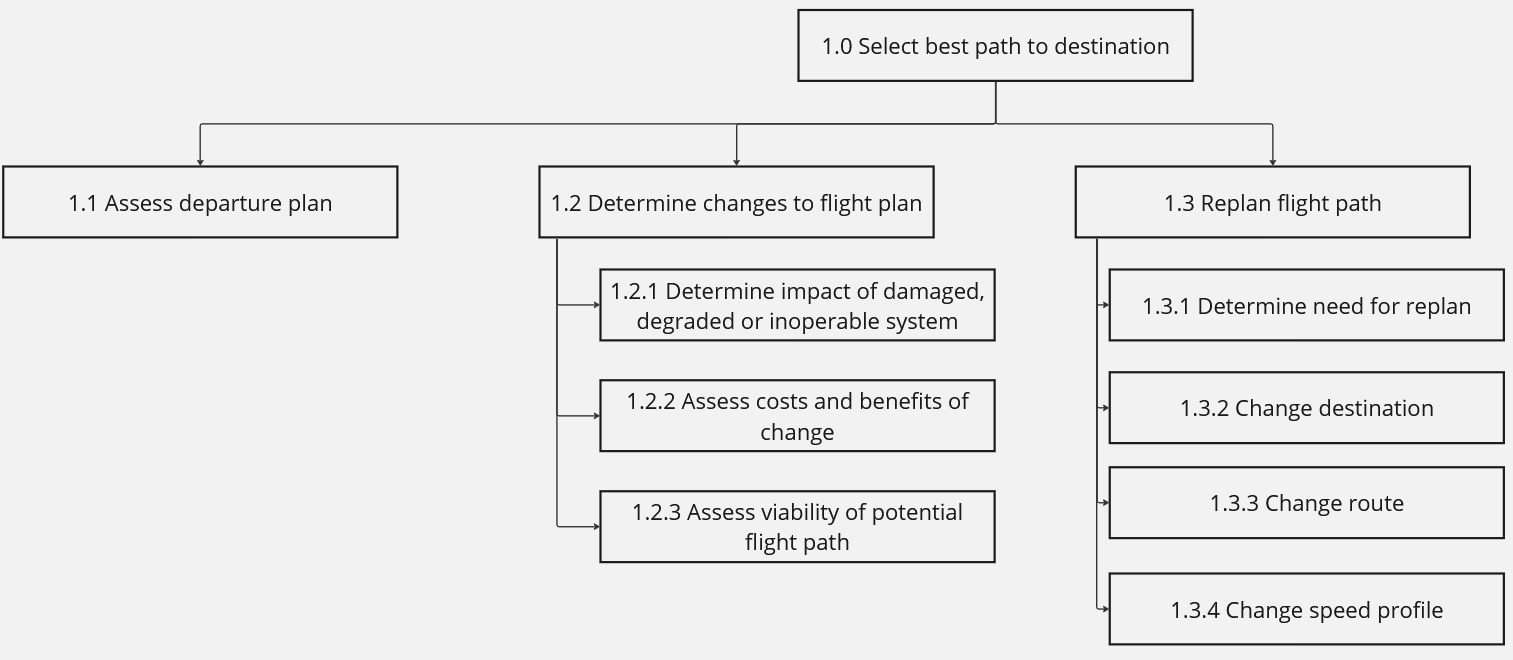
\includegraphics[width=1.0\textwidth]{./images/GDTA/top-goal-1.jpg}
		\label{gdta:top-1}
	\end{figure}

	\begin{figure}[H]
		\centering
		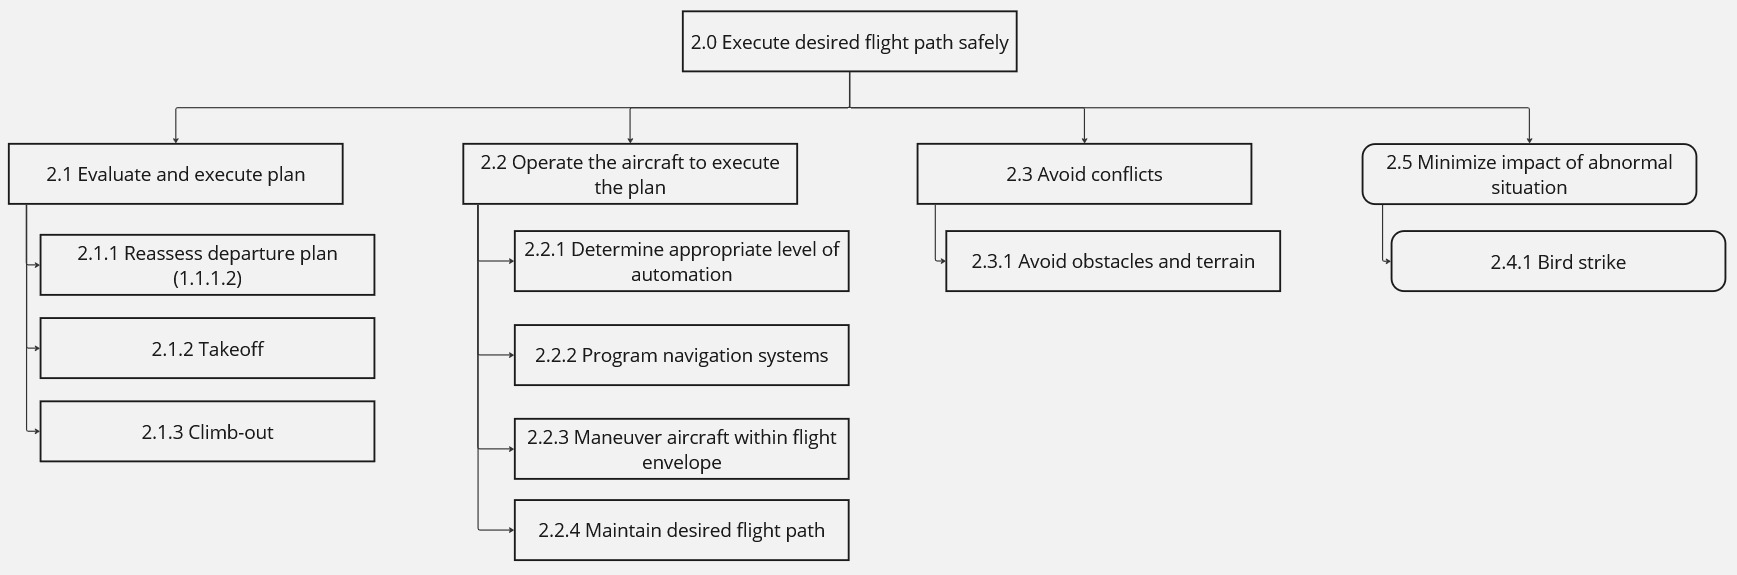
\includegraphics[width=1.0\textwidth]{./images/GDTA/top-goal-2.jpg}
		\label{gdta:top-2}
	\end{figure}

	\begin{figure}[H]
		\centering
		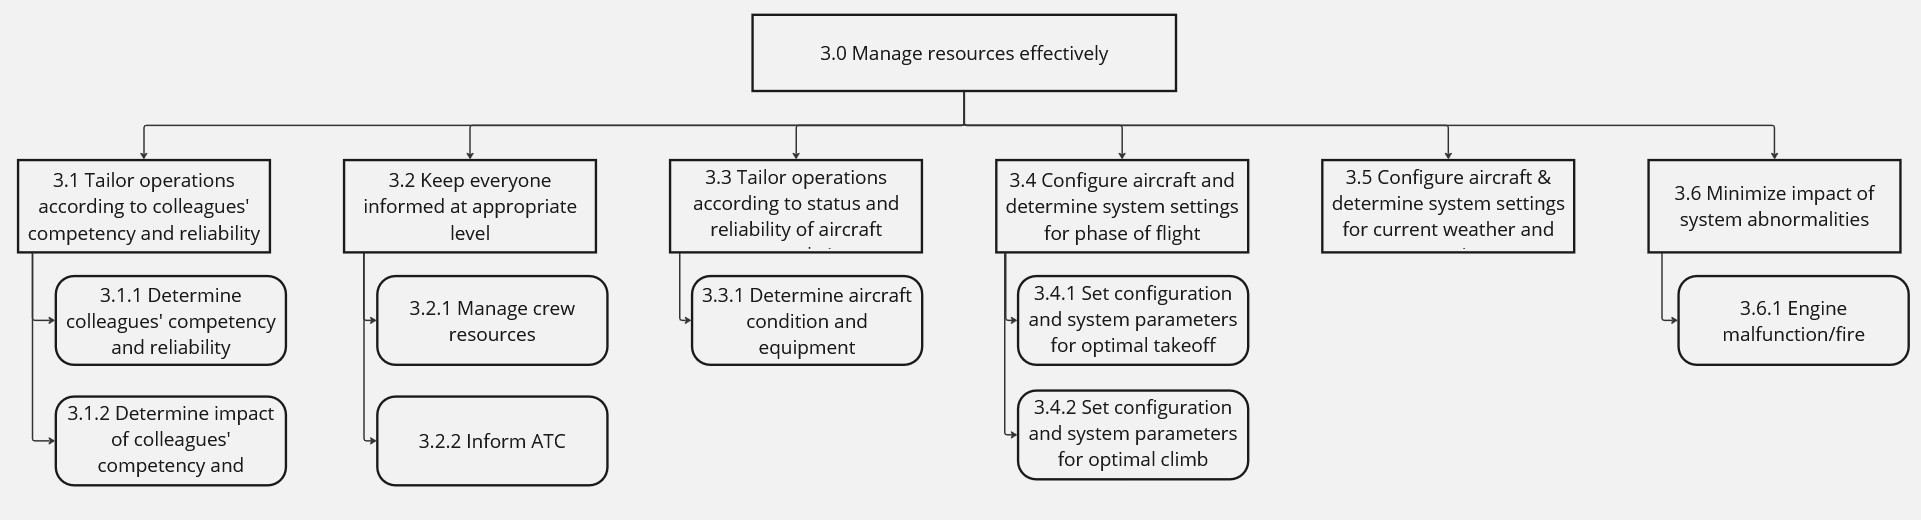
\includegraphics[width=1.0\textwidth]{./images/GDTA/top-goal-3.jpg}
		\label{gdta:top-3}
	\end{figure}

	\subsection{Low-Level Goal hierarchy, SA questions and information requirements}

	\begin{figure}[H]
		\centering
		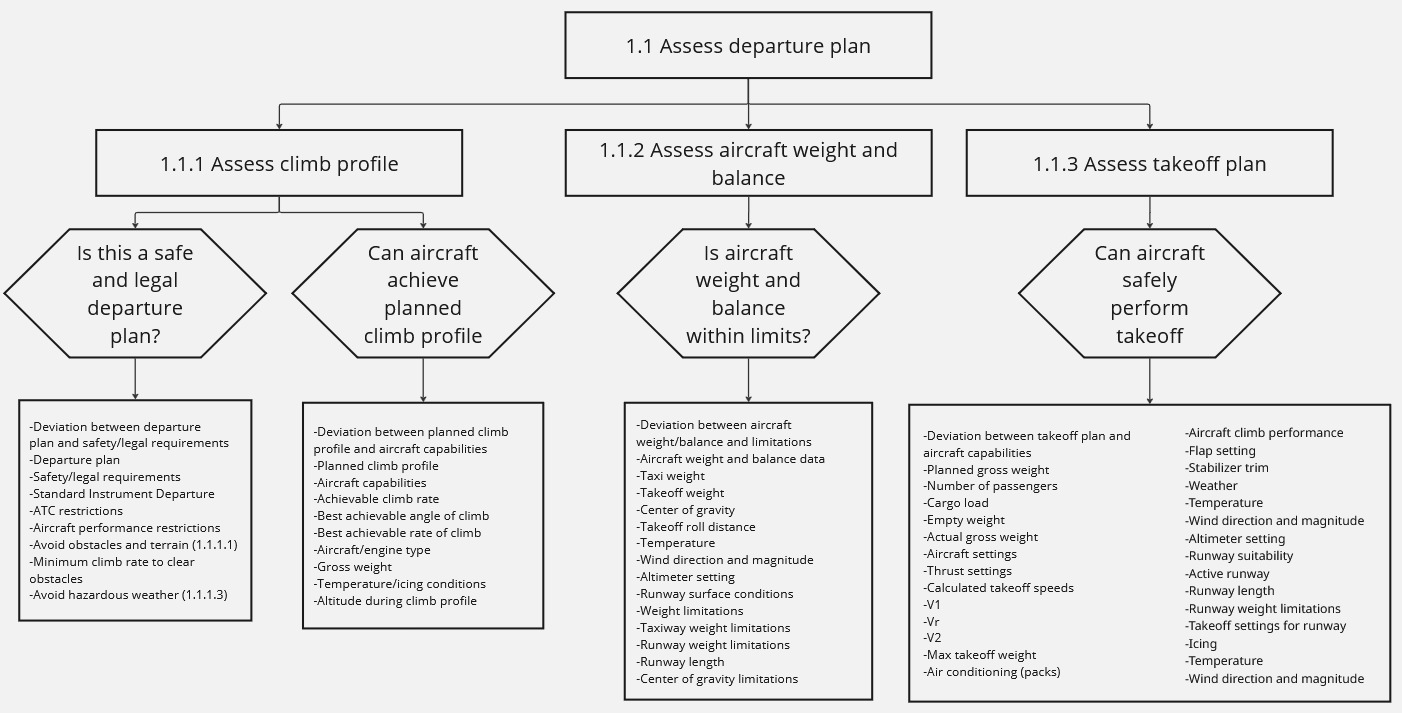
\includegraphics[width=1.0\textwidth]{./images/GDTA/bott-goal-1.jpg}
		\label{gdta:bott-1}
	\end{figure}

	\begin{figure}[H]
		\centering
		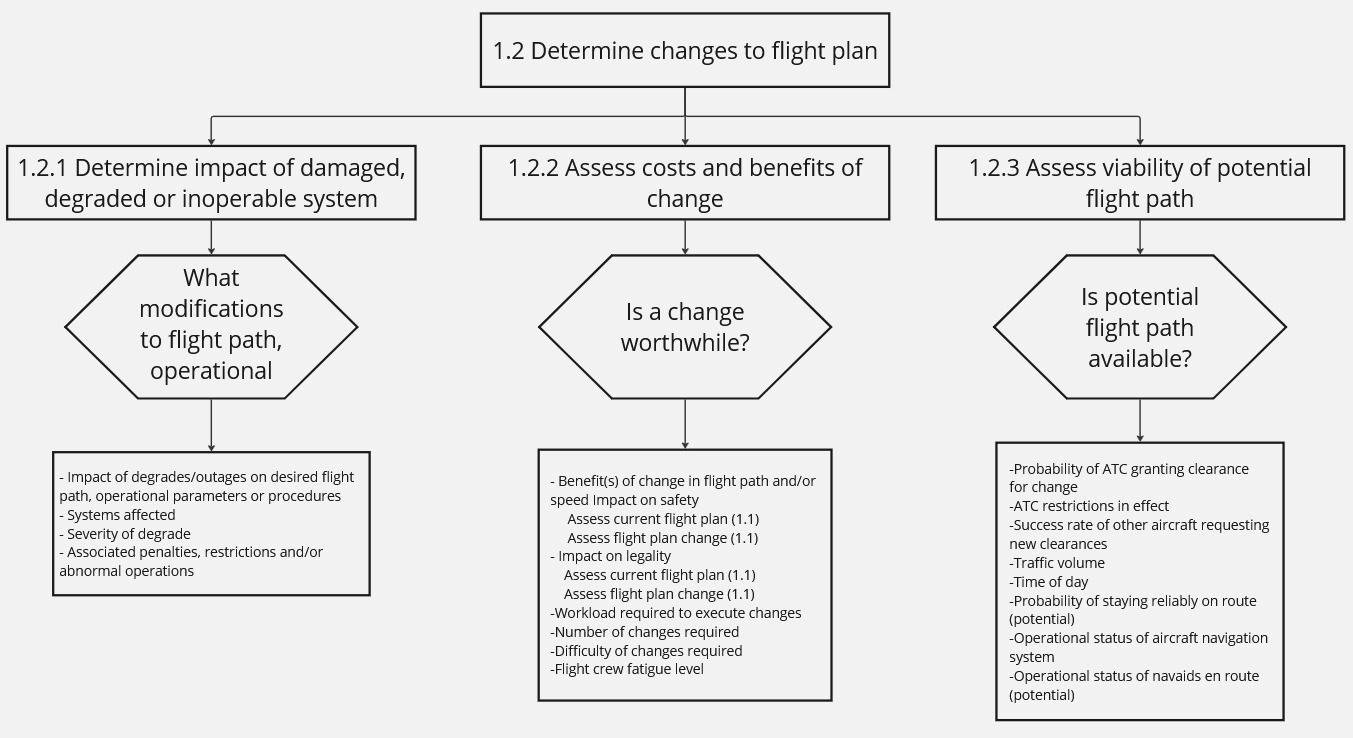
\includegraphics[width=1.0\textwidth]{./images/GDTA/bott-goal-2.jpg}
		\label{gdta:bott-2}
	\end{figure}

	\begin{figure}[H]
		\centering
		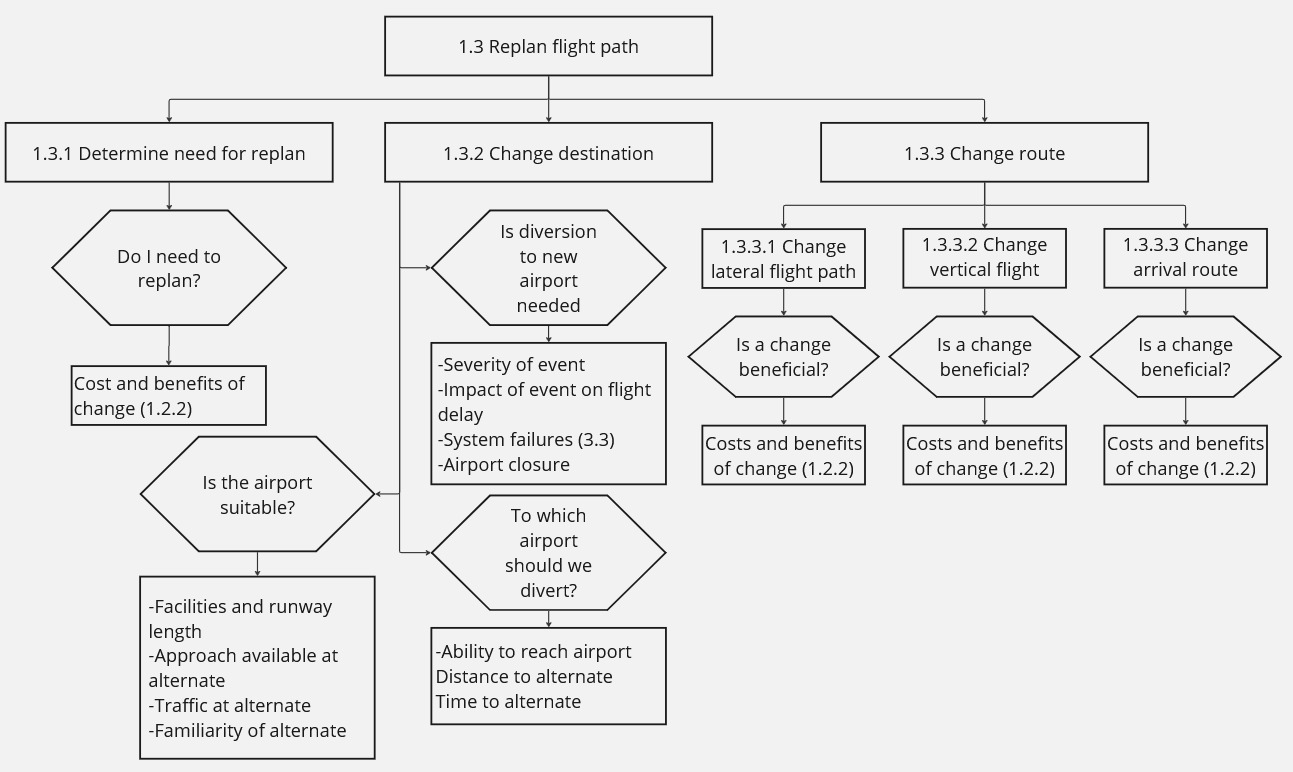
\includegraphics[width=1.0\textwidth]{./images/GDTA/bott-goal-3.jpg}
		\label{gdta:bott-3}
	\end{figure}

	\begin{figure}[H]
		\centering
		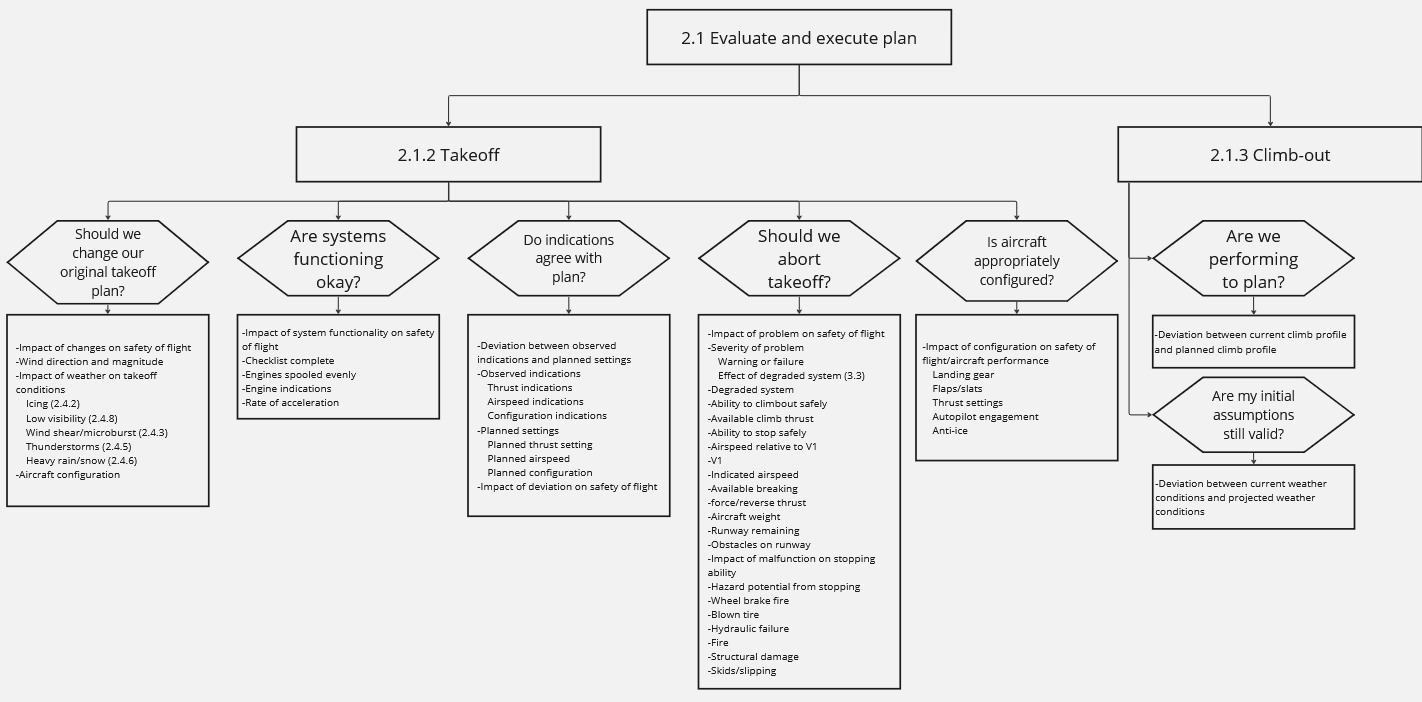
\includegraphics[width=1.0\textwidth]{./images/GDTA/bott-goal-4.jpg}
		\label{gdta:bott-4}
	\end{figure}

	\begin{figure}[H]
		\centering
		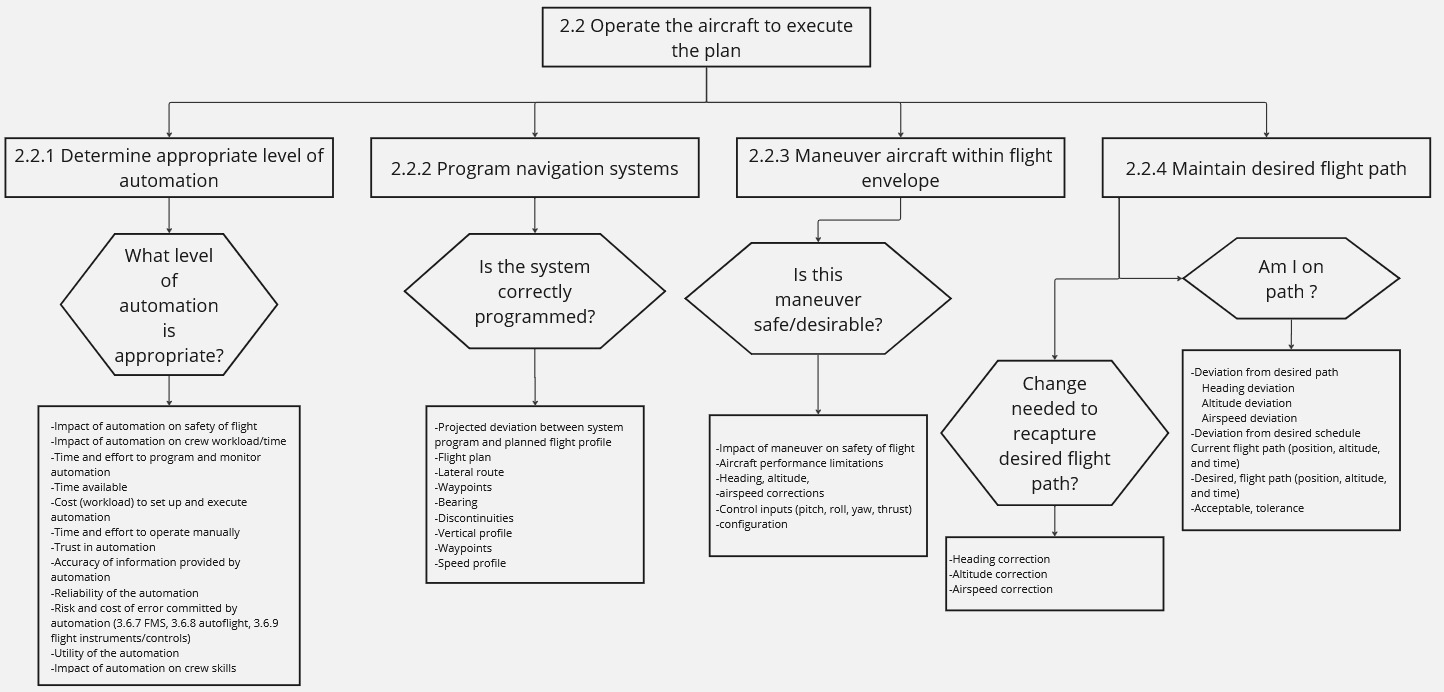
\includegraphics[width=1.0\textwidth]{./images/GDTA/bott-goal-5.jpg}
		\label{gdta:bott-5}
	\end{figure}

	\begin{figure}[H]
		\centering
		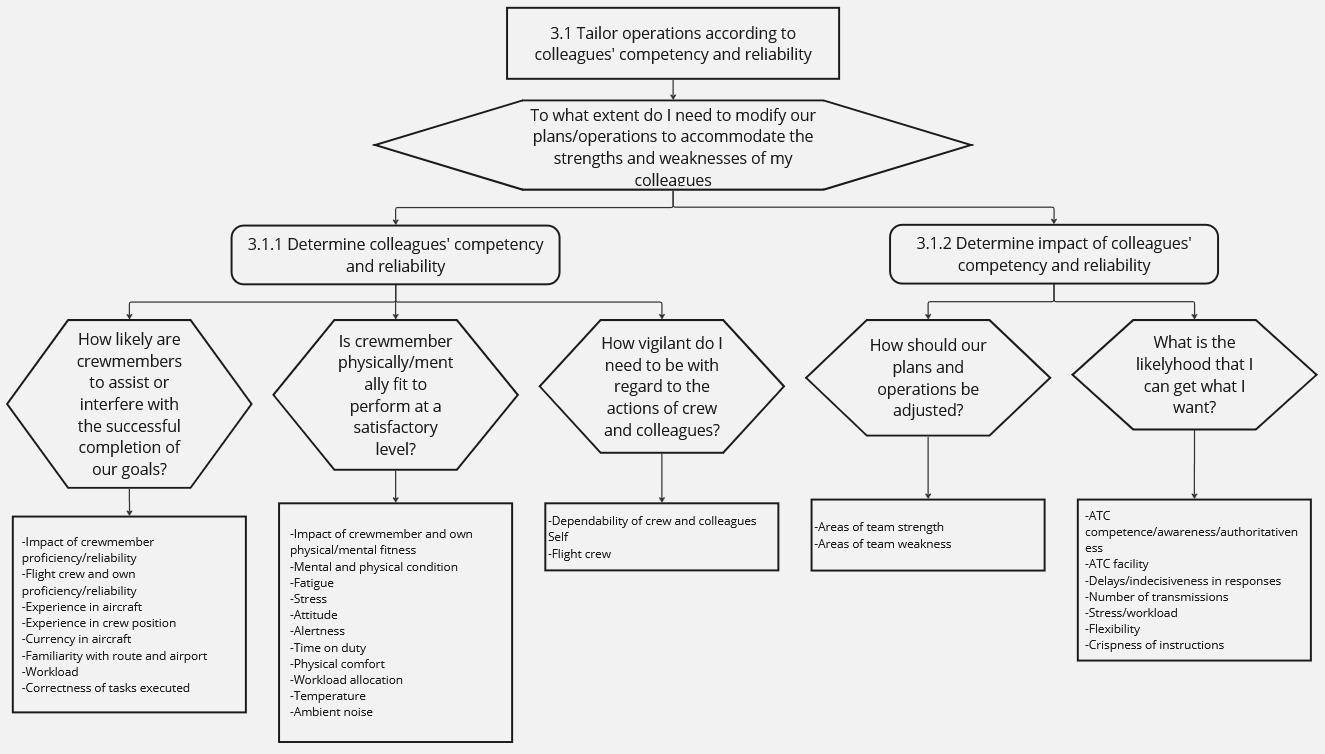
\includegraphics[width=1.0\textwidth]{./images/GDTA/bott-goal-6.jpg}
		\label{gdta:bott-6}
	\end{figure}

	\begin{figure}[H]
		\centering
		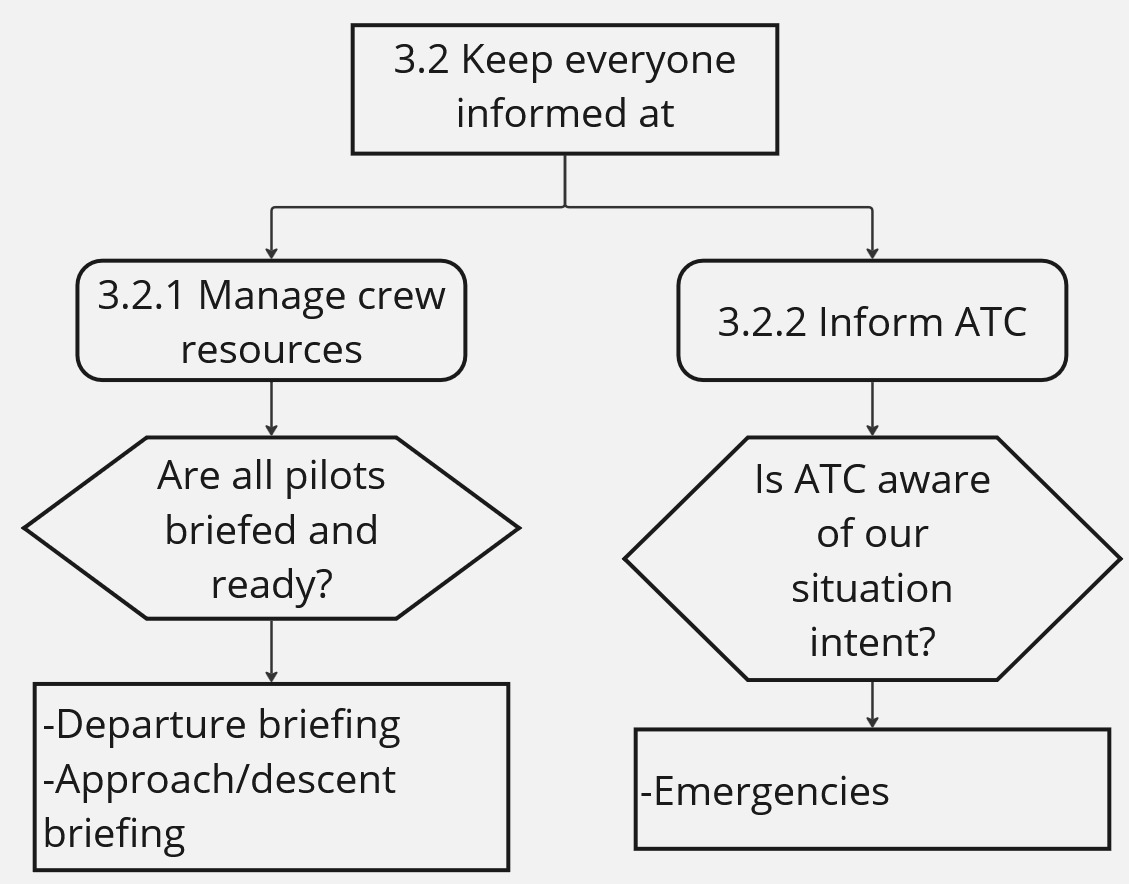
\includegraphics[width=0.8\textwidth]{./images/GDTA/bott-goal-7.jpg}
		\label{gdta:bott-7}
	\end{figure}

	\begin{figure}[H]
		\centering
		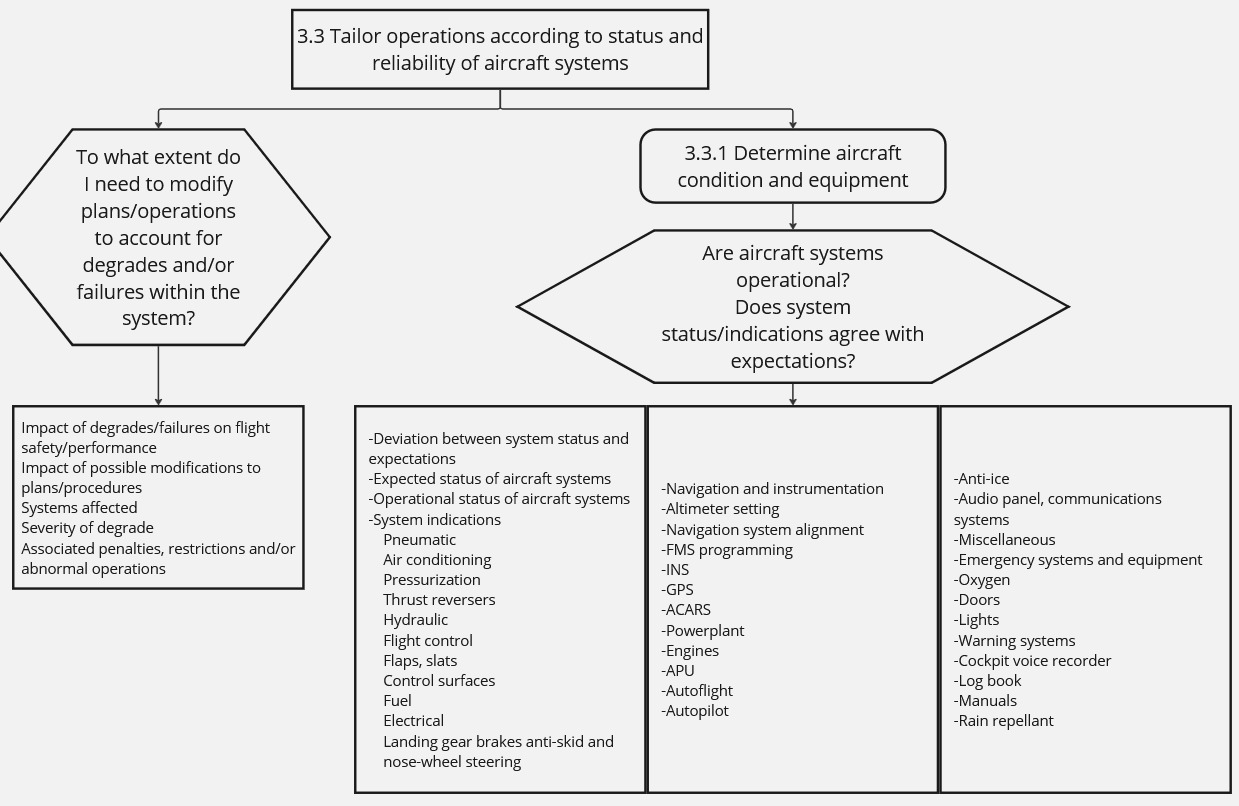
\includegraphics[width=1.0\textwidth]{./images/GDTA/bott-goal-8.jpg}
		\label{gdta:bott-8}
	\end{figure}

	\begin{figure}[H]
		\centering
		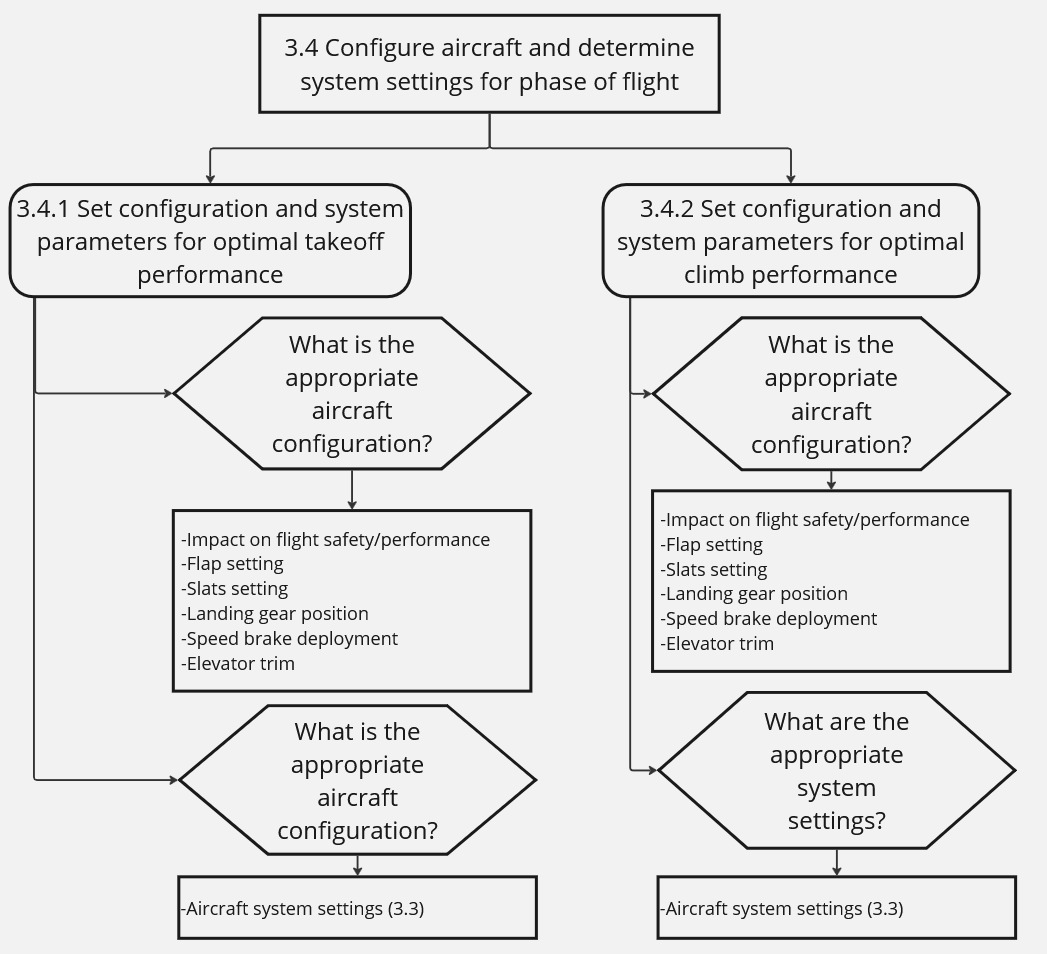
\includegraphics[width=0.8\textwidth]{./images/GDTA/bott-goal-9.jpg}
		\label{gdta:bott-9}
	\end{figure}

	\begin{figure}[H]
		\centering
		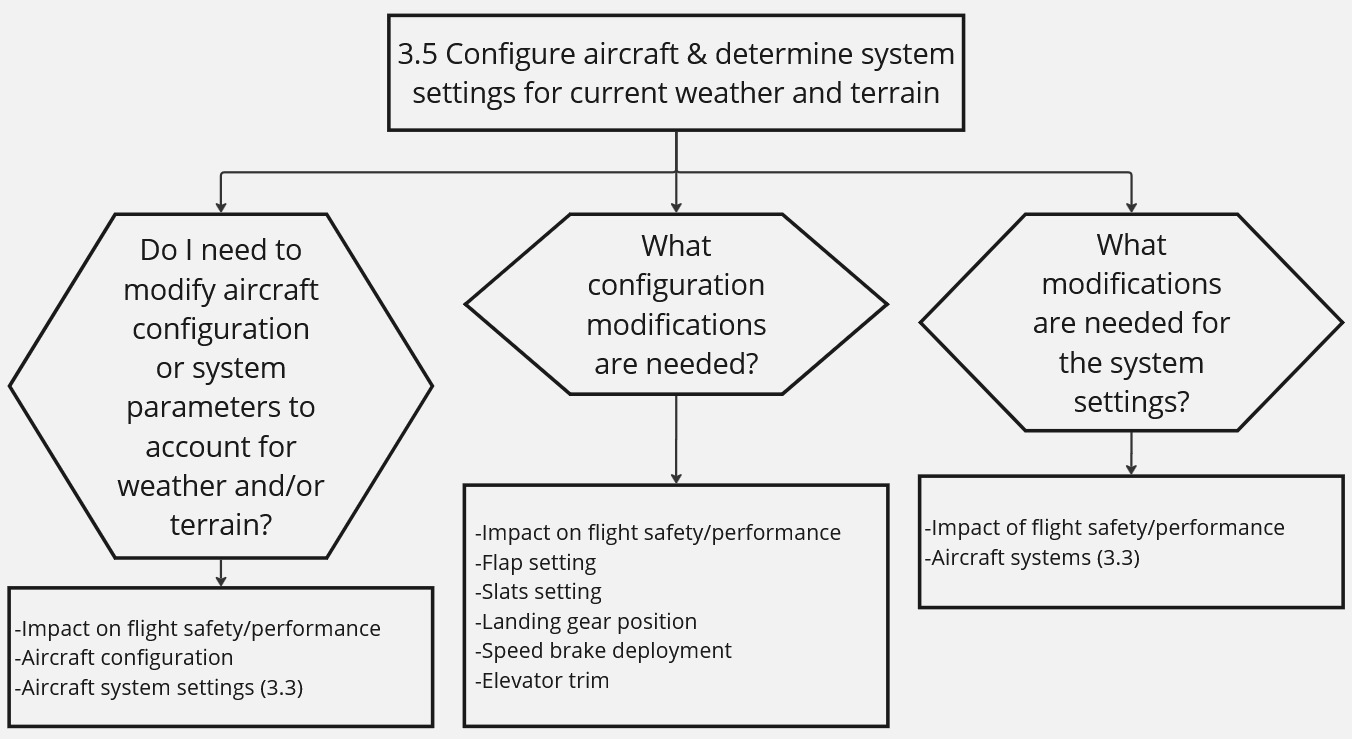
\includegraphics[width=1.0\textwidth]{./images/GDTA/bott-goal-10.jpg}
		\label{gdta:bott-10}
	\end{figure}

	\begin{figure}[H]
		\centering
		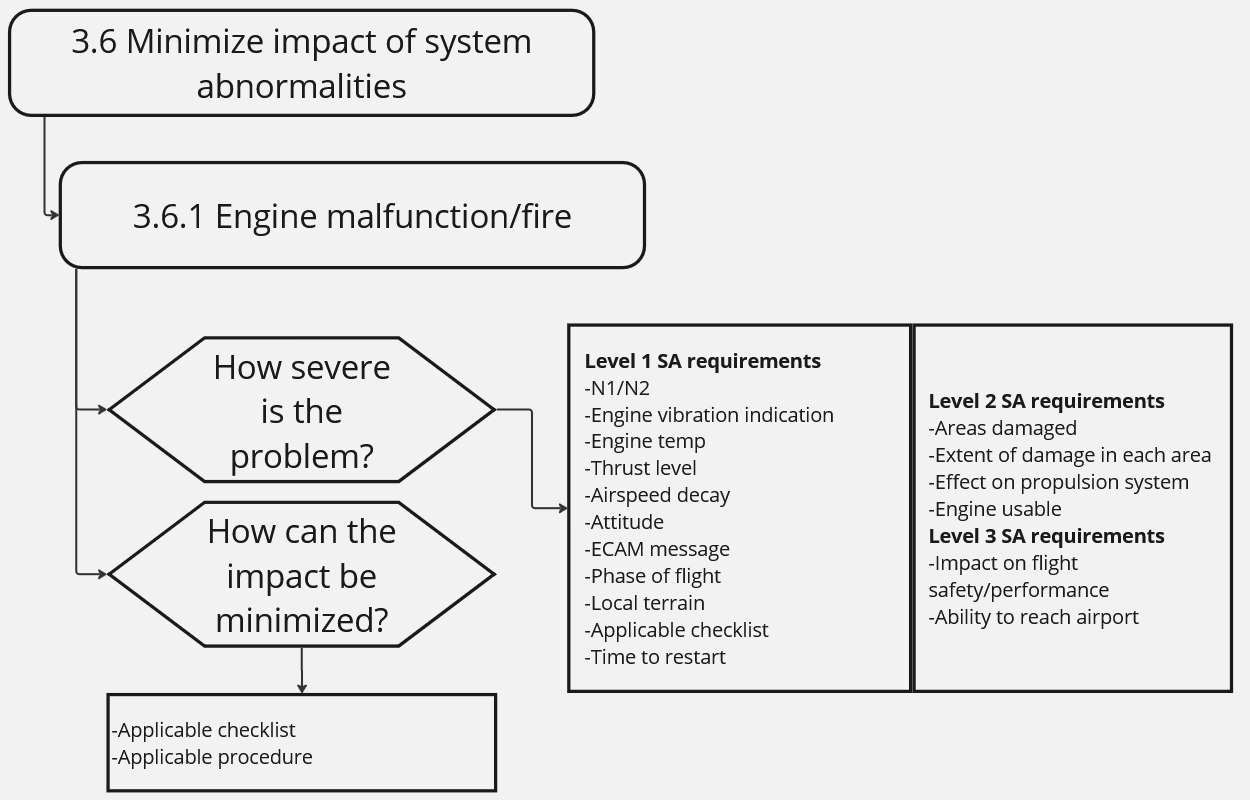
\includegraphics[width=1.0\textwidth]{./images/GDTA/bott-goal-11.jpg}
		\label{gdta:bott-11}
	\end{figure}

	\section{Interdependence Analysis}
	\label{appendix:IA}

	\subsection{Color key for Interdependence Analysis}

	\begin{table}[H]
		\centering
		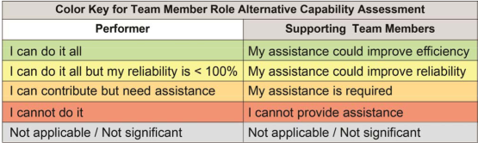
\includegraphics{images/color_key_IA.png}
		\label{table:color-key}
	\end{table}

	\subsection{IA tables}
	\label{table:all-IA}

	\begin{table}[H]
		\centering
		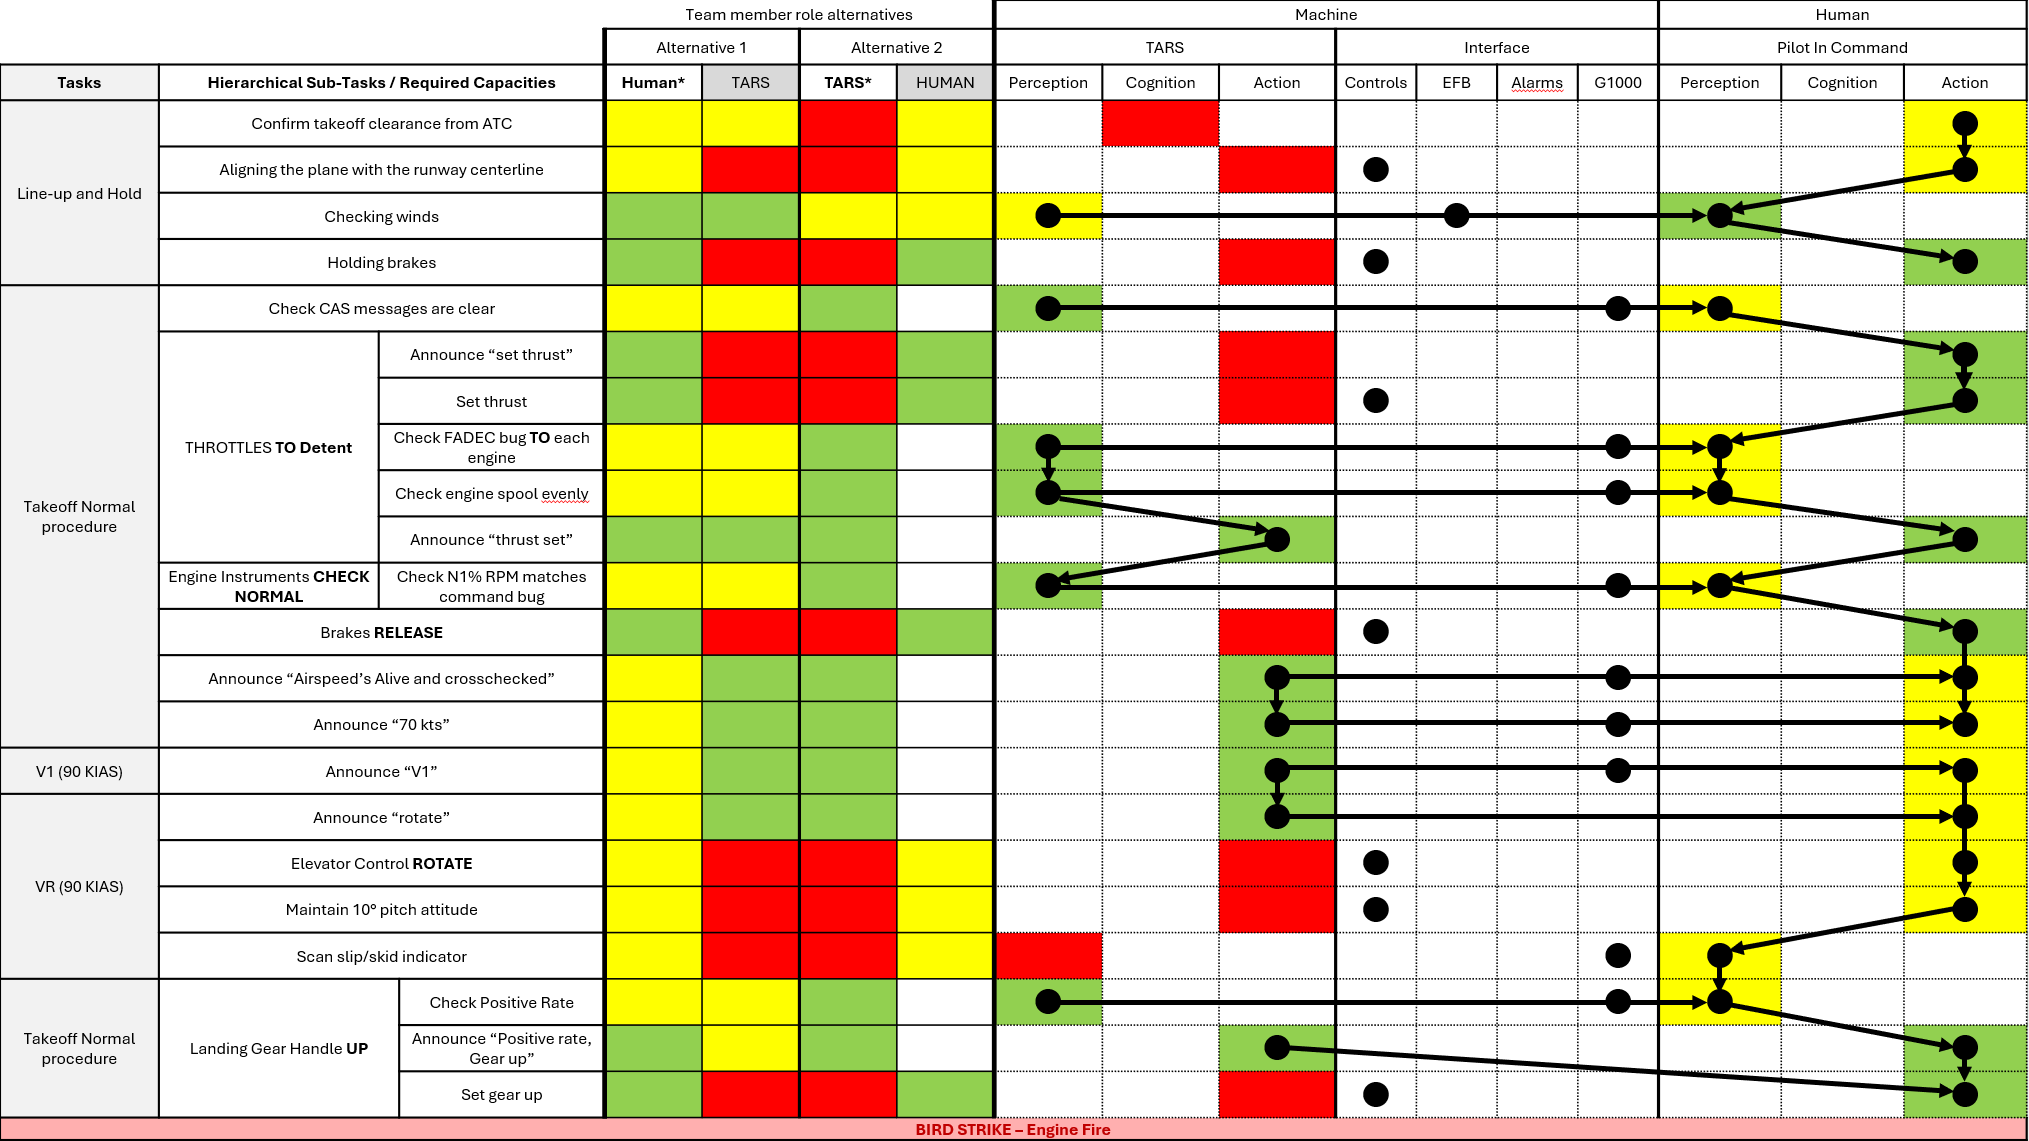
\includegraphics[width=1\textwidth]{images/IA-table-1.png}
	\end{table}

	\begin{table}[H]
		\centering
		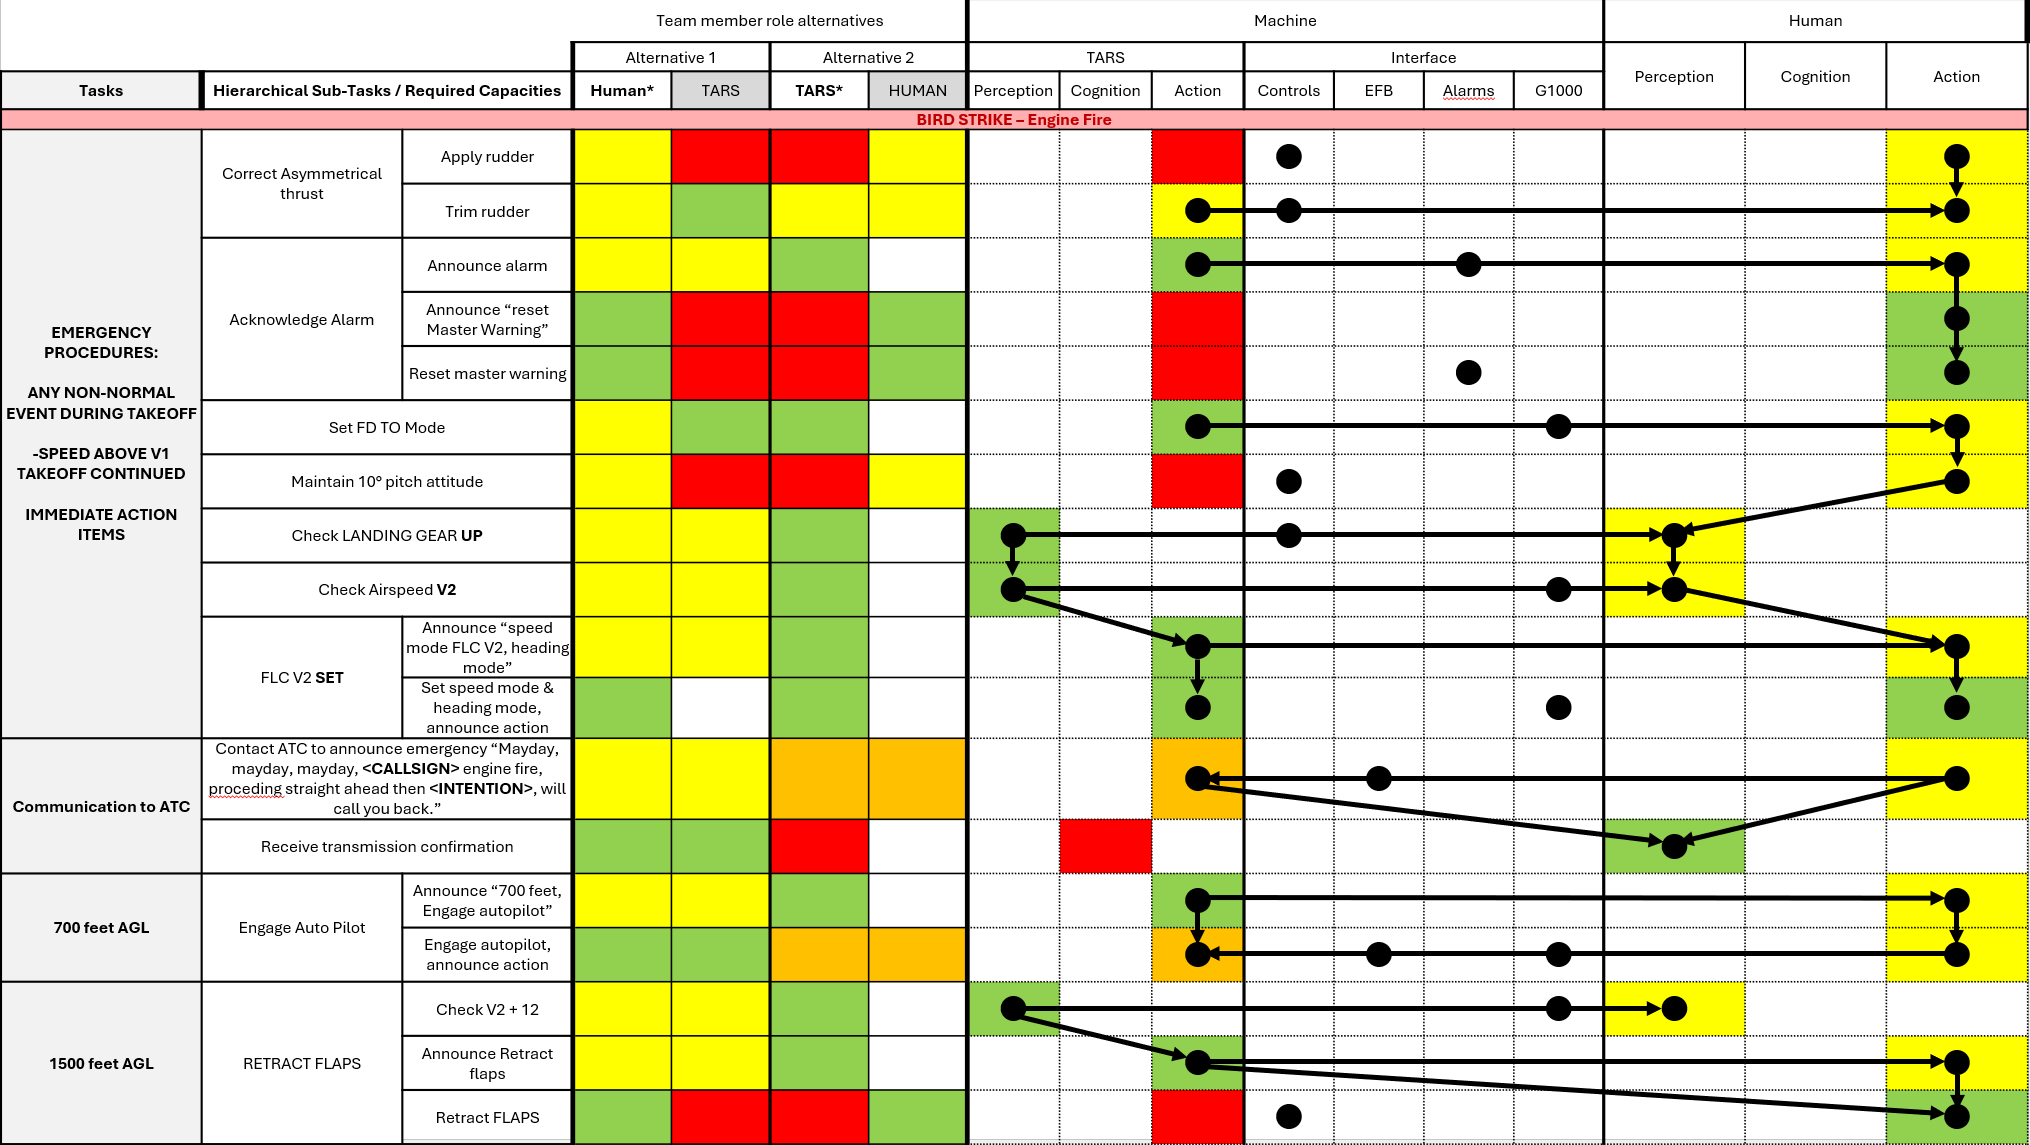
\includegraphics[width=1\textwidth]{images/IA-table-2.png}
	\end{table}

	\begin{table}[H]
		\centering
		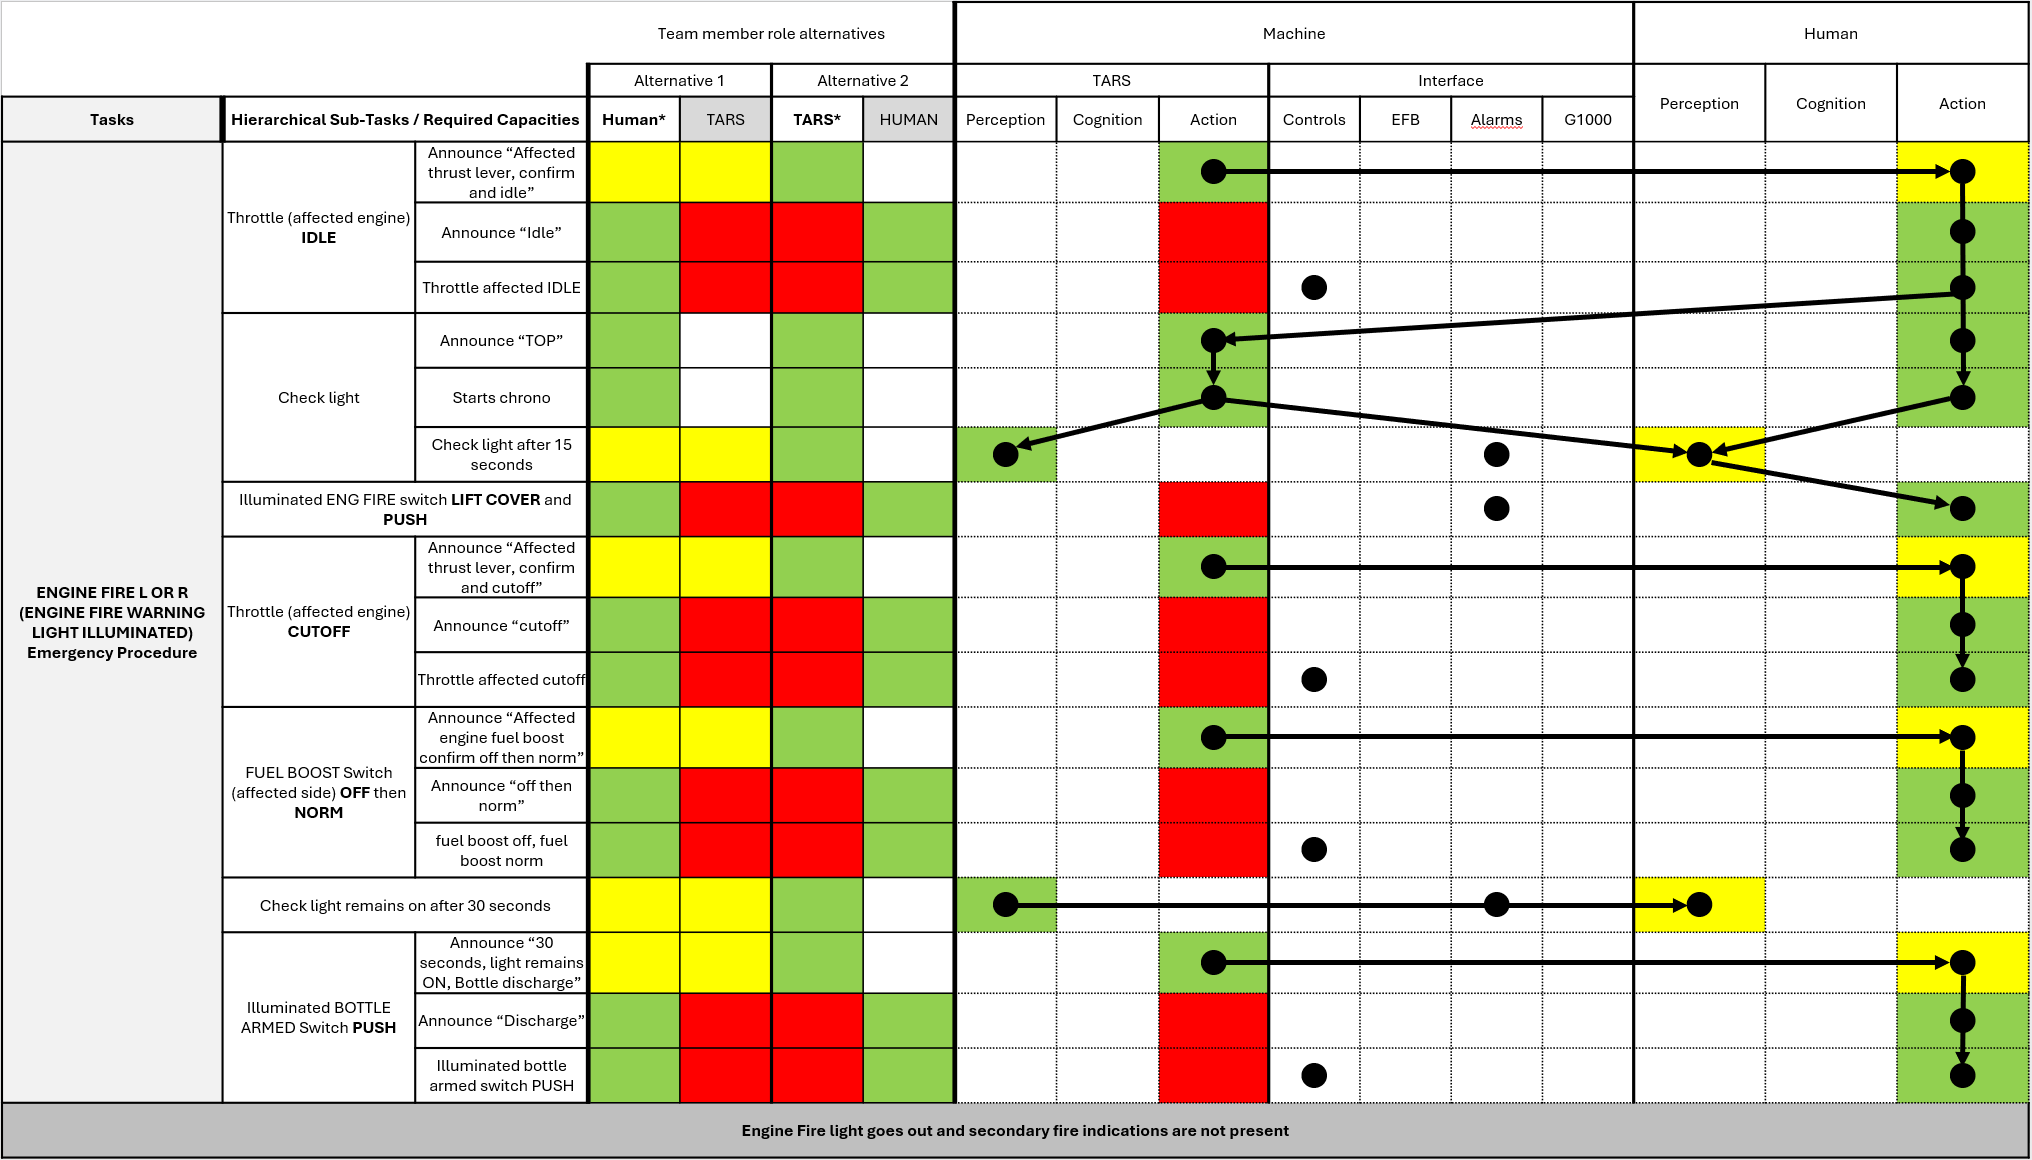
\includegraphics[width=1\textwidth]{images/IA-table-3.png}
	\end{table}

	\begin{table}[H]
		\centering
		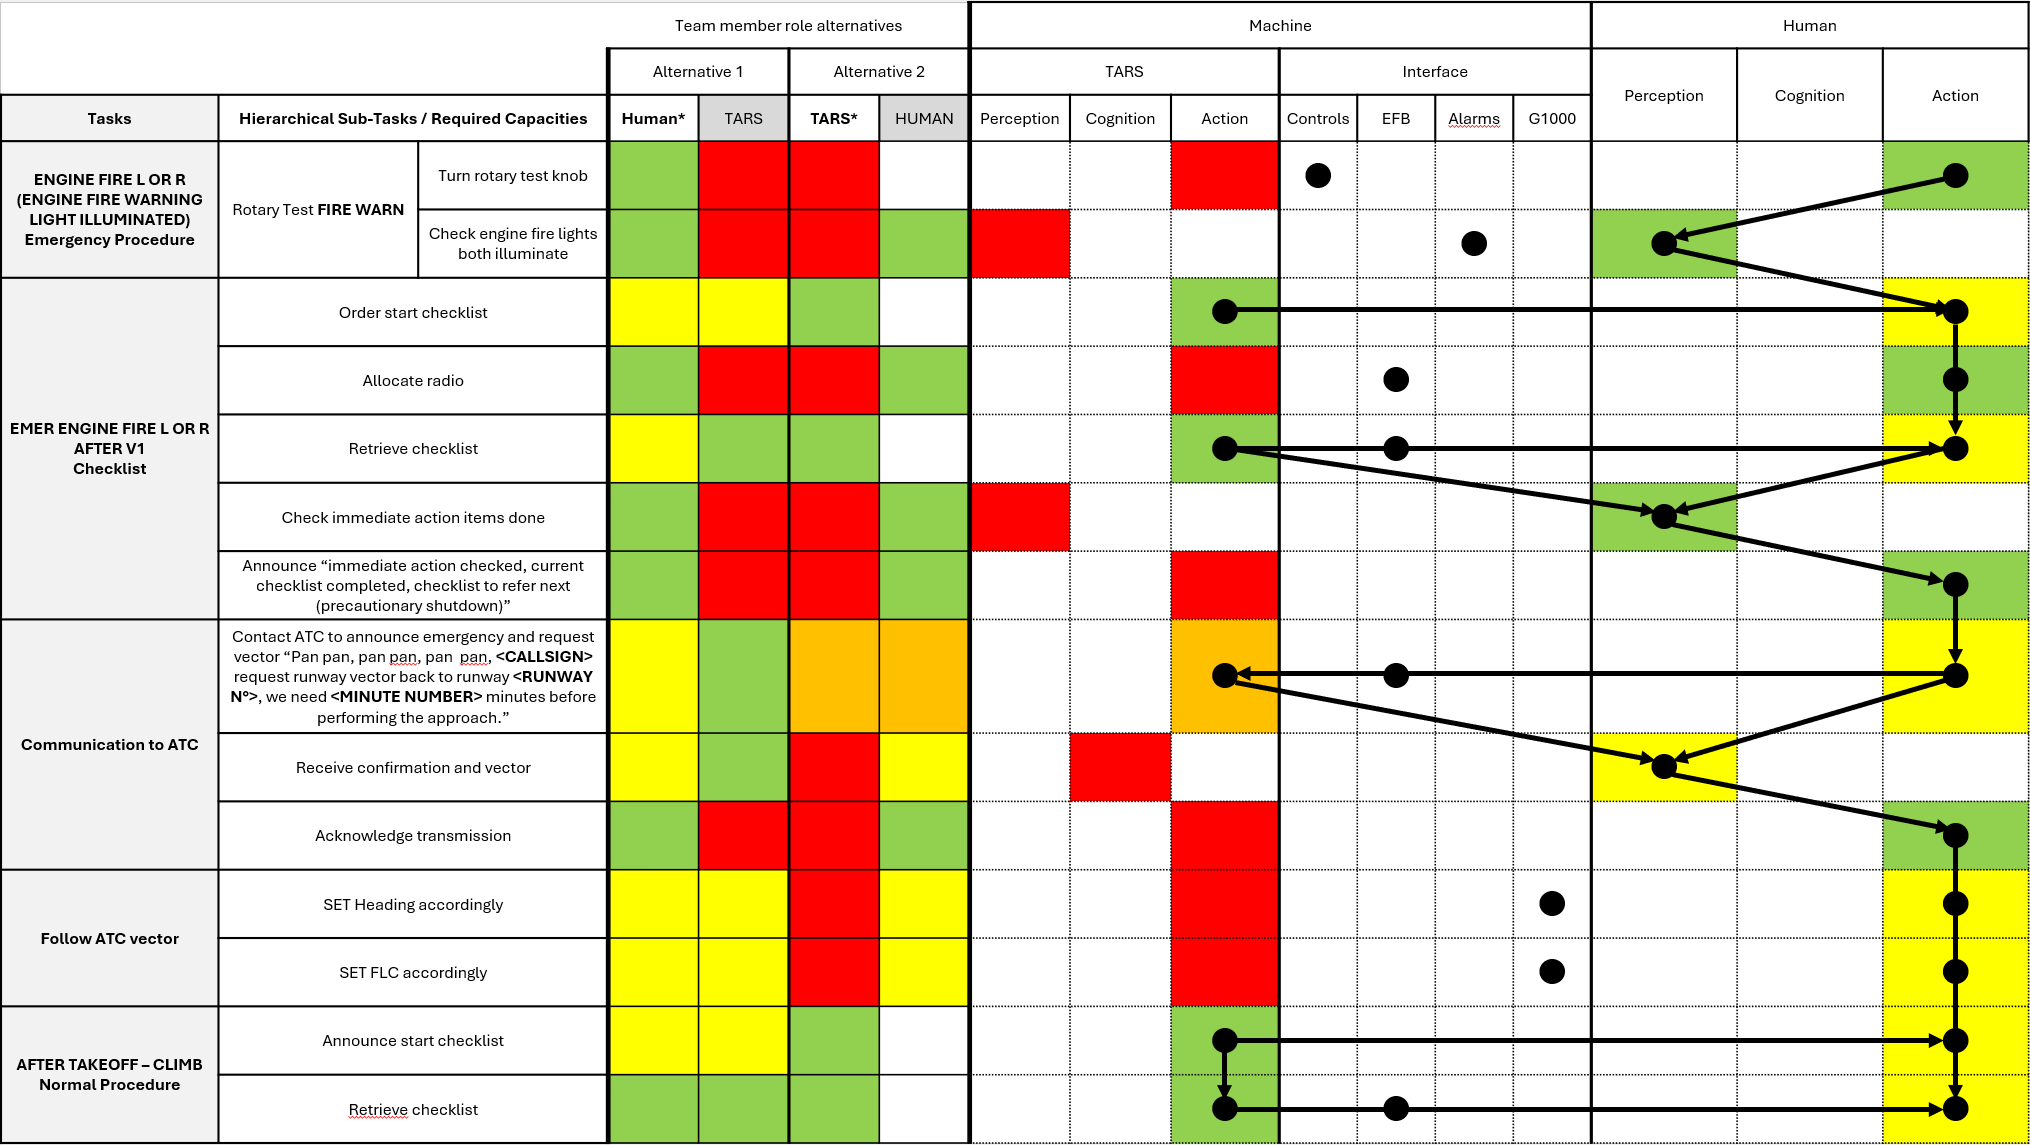
\includegraphics[width=1\textwidth]{images/IA-table-4.png}
	\end{table}

	\begin{table}[H]
		\centering
		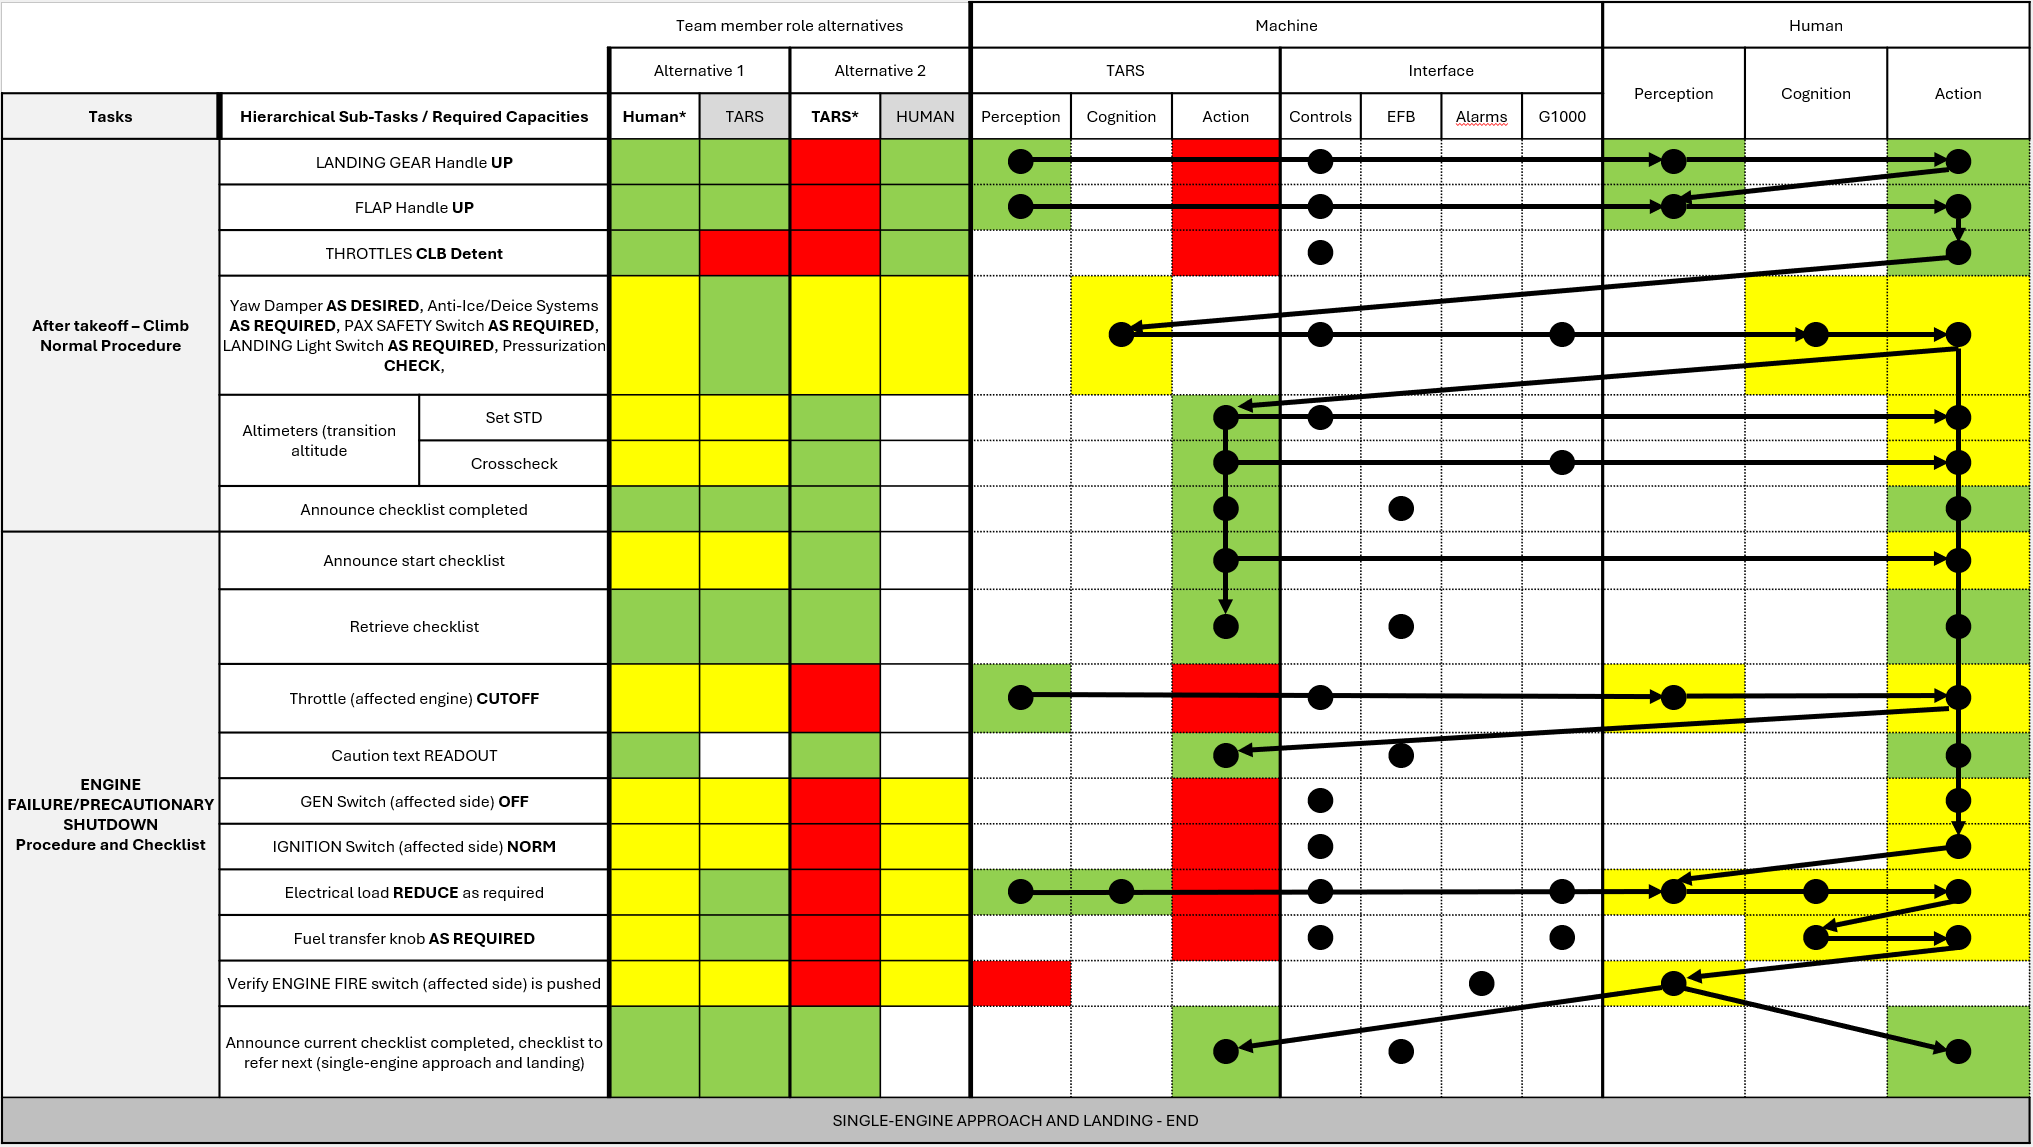
\includegraphics[width=1\textwidth]{images/IA-table-5.png}
	\end{table}

	\printbibliography % Prints the bibliography
\end{document} % Ends the document